\subsubsection{Ստորին գնահատականներ}

$W(K_{2n})$-ի համար նոր ստորին գնահատականներ ստանալու $K_{2n}$-ը տրոհենք երկու կողերով չհատվող կմախքային համասեռ ենթագրաֆների, կառուցենք հատուկ տիպի $1$-ֆակտորիզացիաներ ենթագրաֆներից յուրաքանչյուրի համար, ապա կիրառենք Համարժեքության լեմման այդ $1$-ֆակտորիզացիաների միավորման համար:

Ֆիքսենք $K_{2n}$-ի գագաթների որևէ համարակալում՝ $\mathbf{v} = \left(u_1,v_1, u_2,v_2, \ldots,u_n,v_n\right)$, և սահմանենք $K_{2n}$-ի երկու համասեռ կմախքային ենթագրաֆներ՝ $K_2 \square K_n$ և $K_2 \times K_n$ (Նկ. \ref{K_8products}).
\begin{align*}
&V(K_2 \square K_n) = V(K_2 \times K_n) = V(K_{2n})\\
&E(K_2 \square K_n) = \{u_iu_j : 1\leq i<j \leq n\} \cup \{u_iv_i : 1\leq i \leq n\} \cup \{v_iv_j : 1\leq i<j \leq n\}\\
&E(K_2 \times K_n) = \{u_iv_j : 1\leq i \neq j \leq n\}
\end{align*}


\begin{figure}[b!]
\centering
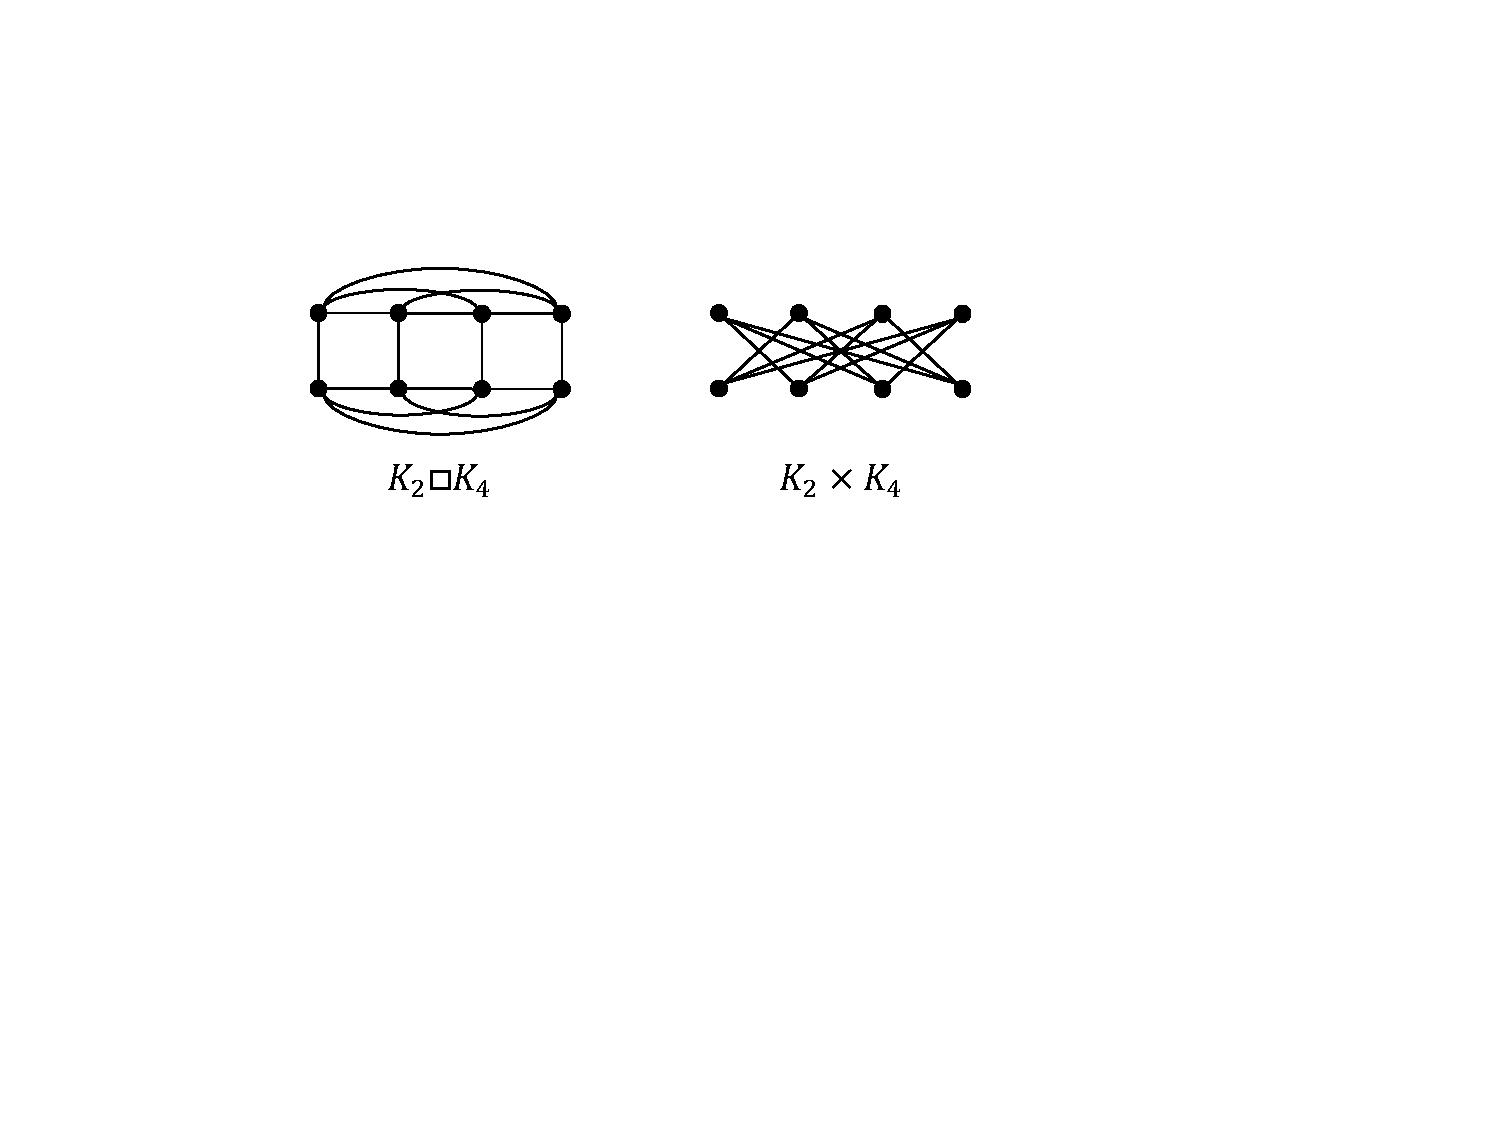
\includegraphics[width=0.43\textwidth]{figures/K_8products.pdf}
\caption{$K_8$-ի երկու համասեռ կմախքային ենթագրաֆներ}
\label{K_8products}
\end{figure}


Նկատենք, որ $E(K_{2n})=E(K_2 \square K_n)\cup E(K_2 \times K_n)$: Ֆիքսված $\mathbf{v} = \left(u_1,v_1, u_2,v_2, \ldots,u_n,v_n\right)$ համարակալման համար կառուցենք $K_2 \square K_n$ գրաֆի հատուկ $1$-ֆակտորիզացիա, որը կնշանակենք $\mathfrak{P}_n$-ով.

$\mathfrak{P}_n = \{P_0, P_1, \ldots, P_{n-1}\}$, որտեղ 
\begin{align*}
P_0 &= \left\{
\begin{tabular}{ll}
$\{u_ju_{n+1-j}, v_jv_{n+1-j} : j=1,2,\ldots,\frac{n}{2}\}$ 
& երբ $n$-ը զույգ է\\
$\{u_ju_{n+1-j}, v_jv_{n+1-j} : j=1,2,\ldots,\lfloor\frac{n}{2}\rfloor\}
\cup \{u_{\frac{n+1}{2}}v_{\frac{n+1}{2}}\}$, & երբ $n$-ը կենտ է\\
\end{tabular}%
\right.
\end{align*}

Բոլոր $i=1,2,\ldots,n-1$, թվերի համար սահմանենք $P_i = l_{\mathbf{v}}^i(P_i) \cup r_{\mathbf{v}}^i(P_i)$, որտեղ
\begin{align*}
l_{\mathbf{v}}^i(P_i) &= \left\{
\begin{tabular}{ll}
$\{u_ju_{i+1-j}, v_jv_{i+1-j} : j=1,2,\ldots,\frac{i}{2}\}$ 
& երբ $i$-ն զույգ է\\
$\{u_ju_{i+1-j}, v_jv_{i+1-j} : j=1,2,\ldots,\lfloor\frac{i}{2}\rfloor\}
\cup \{u_{\frac{i+1}{2}}v_{\frac{i+1}{2}}\}$, & երբ $i$-ն կենտ է\\
\end{tabular}%
\right.\\
r_{\mathbf{v}}^i(P_i) &= \left\{
\begin{tabular}{ll}
$\{u_{i+j}u_{n+1-j}, v_{i+j}v_{n+1-j} : j=1,2,\ldots,\frac{n-i}{2}\}$ 
& երբ $n-i$ զույգ է\\
$\{u_{i+j}u_{n+1-j}, v_{i+j}v_{n+1-j} : j=1,2,\ldots,\lfloor\frac{n-i}{2}\rfloor\}
\cup \{u_{\frac{n+i+1}{2}}v_{\frac{n+i+1}{2}}\}$, & երբ $n-i$ կենտ է\\
\end{tabular}%
\right.
\end{align*}

\begin{figure}[t!]
\centering
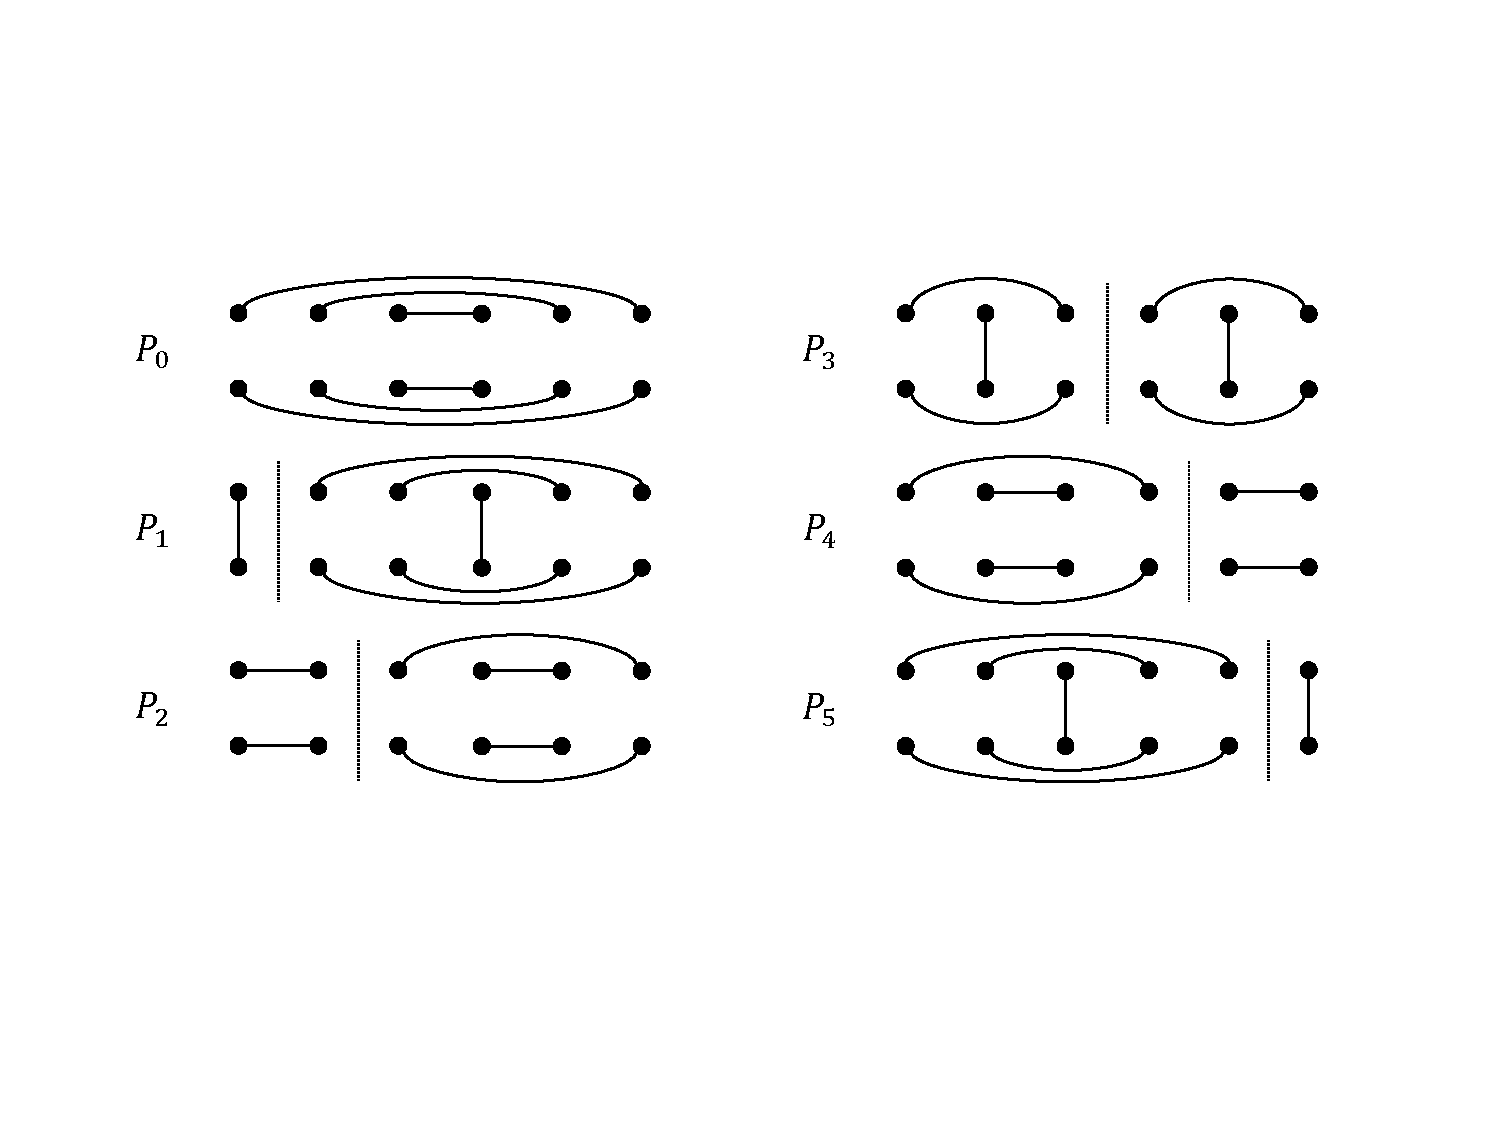
\includegraphics[width=0.7\textwidth]{figures/P_6.pdf}
\caption{$K_2 \square K_6$-ի $\mathfrak{P}_6$ $1$-ֆակտորիզացիան}
\label{P_6}
\end{figure}


Պարզ է, որ $P_i$-ն $i$-բաժանված կատարյալ զուգակցում է բոլոր $i=1,2,\ldots,n-1$ թվերի համար: Նկատենք, որ $K_2 \times K_n$-ը համասեռ երկկողմանի գրաֆ է, ուստի ըստ Քյոնիգի թեորեմի \cite{Konig1916} այն ունի $1$-ֆակտորիզացիա: Եթե $K_2 \times K_n$-ի $1$-ֆակտորիզացիայի բոլոր կատարյալ զուգակցումները համարենք չտրոհված զուգակցումներ և ավելացնենք $\mathfrak{P}_n$-ի կատարյալ զուգակցումները, ապա կստանանք, որ $\sigma_n \geq n-1$: Համարժեքության թեորեմից հետևում է, որ այս արդյունքը համարժեք է Թեորեմ \ref{tPetrosyan3n2}-ին: 

Այս ստորին գնահատականը լավացնելու համար փորձենք կառուցել $K_2 \times K_n$-ի ավելի լավ $1$-ֆակտորիզացիա:

\begin{lemma}\label{l35n3}
Եթե $n \geq 2$, ապա $\sigma_n \geq \lfloor 1.5n \rfloor - 2$:
\end{lemma}
\begin{proof}[Ապացույց]
Ֆիքսենք գագաթների $\mathbf{v} = \left(u_1,v_1,u_2,v_2,\ldots,u_n,v_n\right)$ համարակալումը և դիտարկենք երկու ծնված ենթագրաֆներ.
\begin{align*}
G_1 &= K_2 \times K_n\left[\left\{u_1,v_1,u_2,v_2,\ldots,u_{\lfloor\frac{n}{2}\rfloor},v_{\lfloor\frac{n}{2}\rfloor}\right\}\right]\\ 
G_2 &= K_2 \times K_n\left[\left\{u_{\lfloor\frac{n}{2}\rfloor + 1},v_{\lfloor\frac{n}{2}\rfloor + 1},
u_{\lfloor\frac{n}{2}\rfloor + 2},v_{\lfloor\frac{n}{2}\rfloor + 2},\ldots,u_n,v_n \right\}\right]
\end{align*}
Երկու ենթագրաֆերն էլ համասեռ են ու երկկողմանի, հետևաբար ըստ Քյոնիգի թեորեմի \cite{Konig1916} ունեն $1$-ֆակտորիզացիա: Դիցուք $G_1$-ի և $G_2$-ի $1$-ֆակտորիզացիաներն են համապատասխանաբար $F^l_1,F^l_2,\ldots,F^l_{\lfloor\frac{n}{2}\rfloor-1}$ և $F^r_1,F^r_2,\ldots,F^r_{\lceil\frac{n}{2}\rceil-1}$: Միավորելով այս զուգակցումների առաջին $\lfloor\frac{n}{2}\rfloor-1$ զույգերը, կստանանք $K_2 \times K_n$-ի $\lfloor\frac{n}{2}\rfloor$-բաժանված կատարյալ զուգակցումներ $\mathbf{v}$ համարակալման նկատմամբ.

\begin{center}
$F_i = F^l_i \cup F^r_i$, բոլոր $i=1,2,\ldots,\lfloor\frac{n}{2}\rfloor - 1$ թվերի համար:
\end{center}

Եթե $K_2 \times K_n$ գրաֆից հանենք $\bigcup\limits_{i=1}^{\lfloor\frac{n}{2}\rfloor-1}F_i$ կողերը, ստացված գրաֆը ևս համասեռ երկկողմանի է և ունի $1$-ֆակտորիզացիա, որը նշանակենք $\mathfrak{F}_0$-ով: Ստացվում է, որ $\mathfrak{F}_0 \cup \bigcup\limits_{i=1}^{\lfloor\frac{n}{2}\rfloor-1}F_i \cup \mathfrak{P}_n$ $K_{2n}$-ի $1$-ֆակտորիզացիա է: Բաժանված կատարյալ զուգակցումների քանակը $\lfloor\frac{n}{2}\rfloor - 1 + n - 1$ է: Ուստի ստանում ենք, որ $\sigma_n \geq \lfloor 1.5n \rfloor - 2$:
\end{proof}

Կիրառելով Համարժեքության թեորեմը՝ ստանում ենք հետևյալ ստորին գնահատականը.
\begin{theorem}
\label{t35n3}
Եթե $n \geq 2$, ապա $W(K_{2n}) \geq \lfloor 3.5n \rfloor - 3$:
\end{theorem}

Այս թեորեմից հետևում է, որ $W(K_{10}) \geq 14$, որը Հիպոթեզ \ref{h1_complete_pq}-ը հերքող ամենափոքր օրինակն է: Այսուհետ կքննարկենք այն դեպքը, երբ $n$-ը բաղադրյալ թիվ է:

\begin{lemma}\label{lComposite}
Ցանկացած $m,n \in\mathbb{N}$ թվերի համար $\sigma_{mn} \geq \sigma_m + \sigma_n + 2(m-1)(n-1)$:
\end{lemma}
\begin{proof}[Ապացույց]
Նշանակենք $K_{2mn}$, $K_{2n}$ և $K_{2m}$ գրաֆների գագաթների բազմությունը հետևյալ կերպ.
\begin{align*}
V(K_{2mn}) &= \left\{u_i^j,v_i^j : i=1,2,\ldots,n,\ j=1,2,\ldots,m\right\} \\
V(K_{2n}) &= \left\{\overline{u}_i,\overline{v}_i : i=1,2,\ldots,n \right\} \\ 
V(K_{2m}) &= \left\{\widetilde{u}^i,\widetilde{v}^i : i=1,2,\ldots,m \right\} 
\end{align*}


\begin{figure}[t!]
\centering
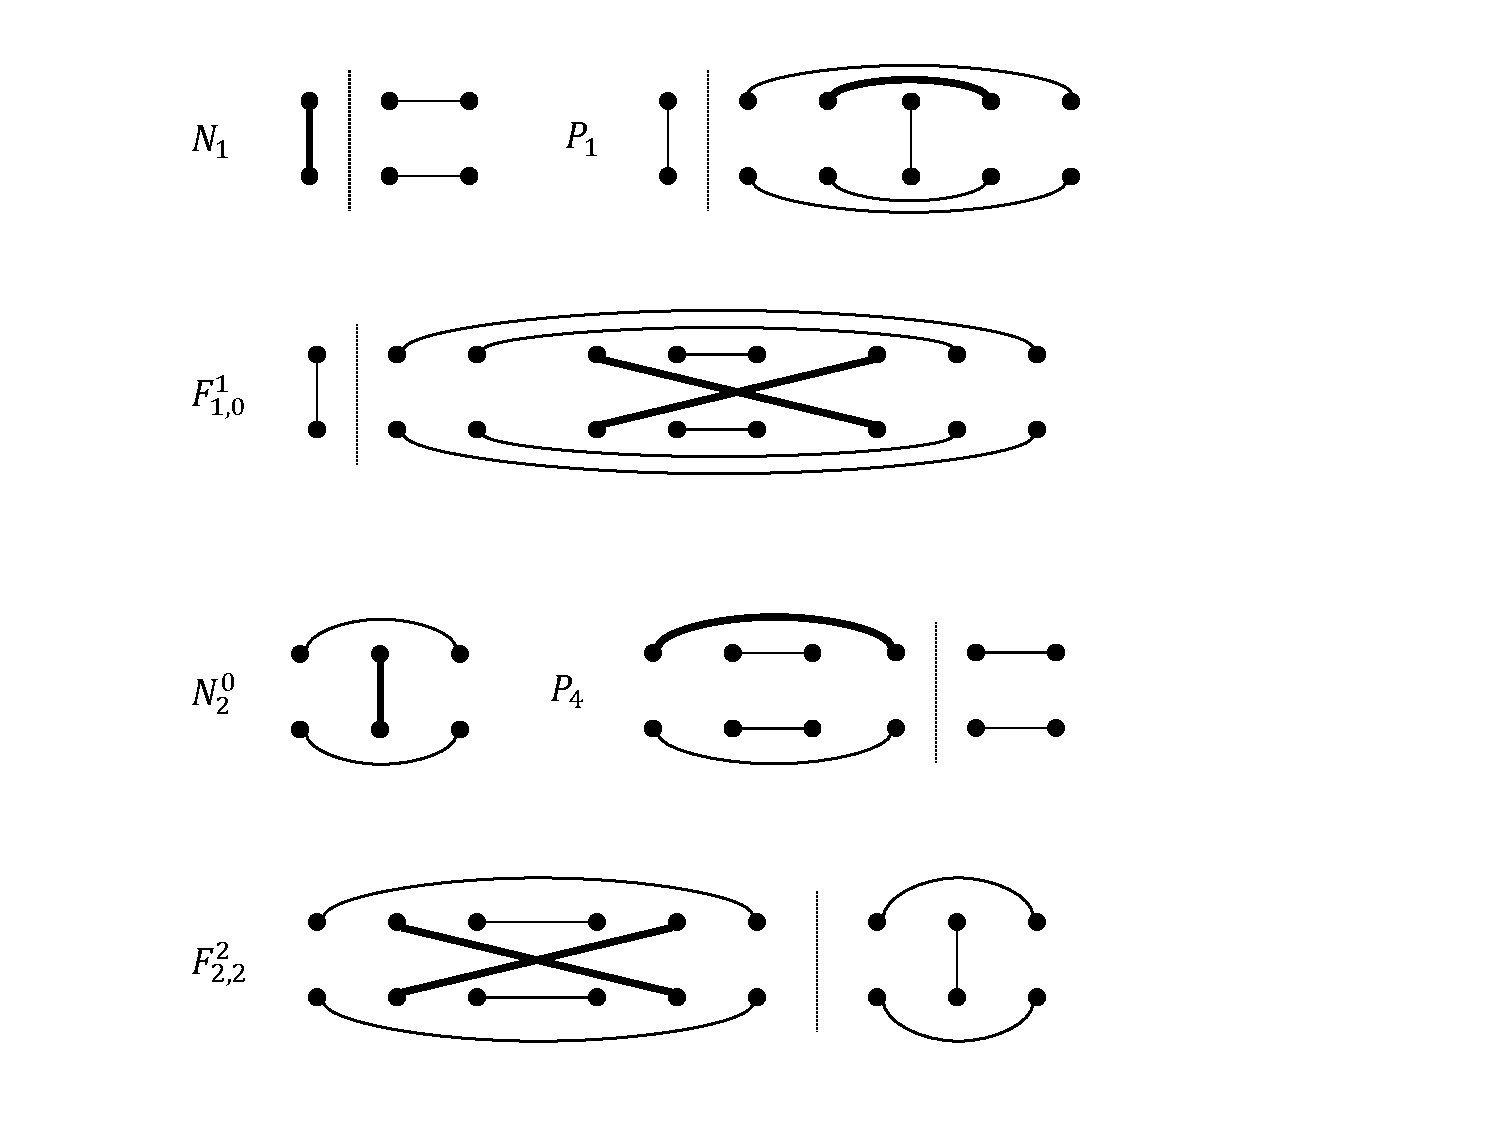
\includegraphics[width=0.39\textwidth]{figures/K_18-1.pdf}
\hspace{1cm}
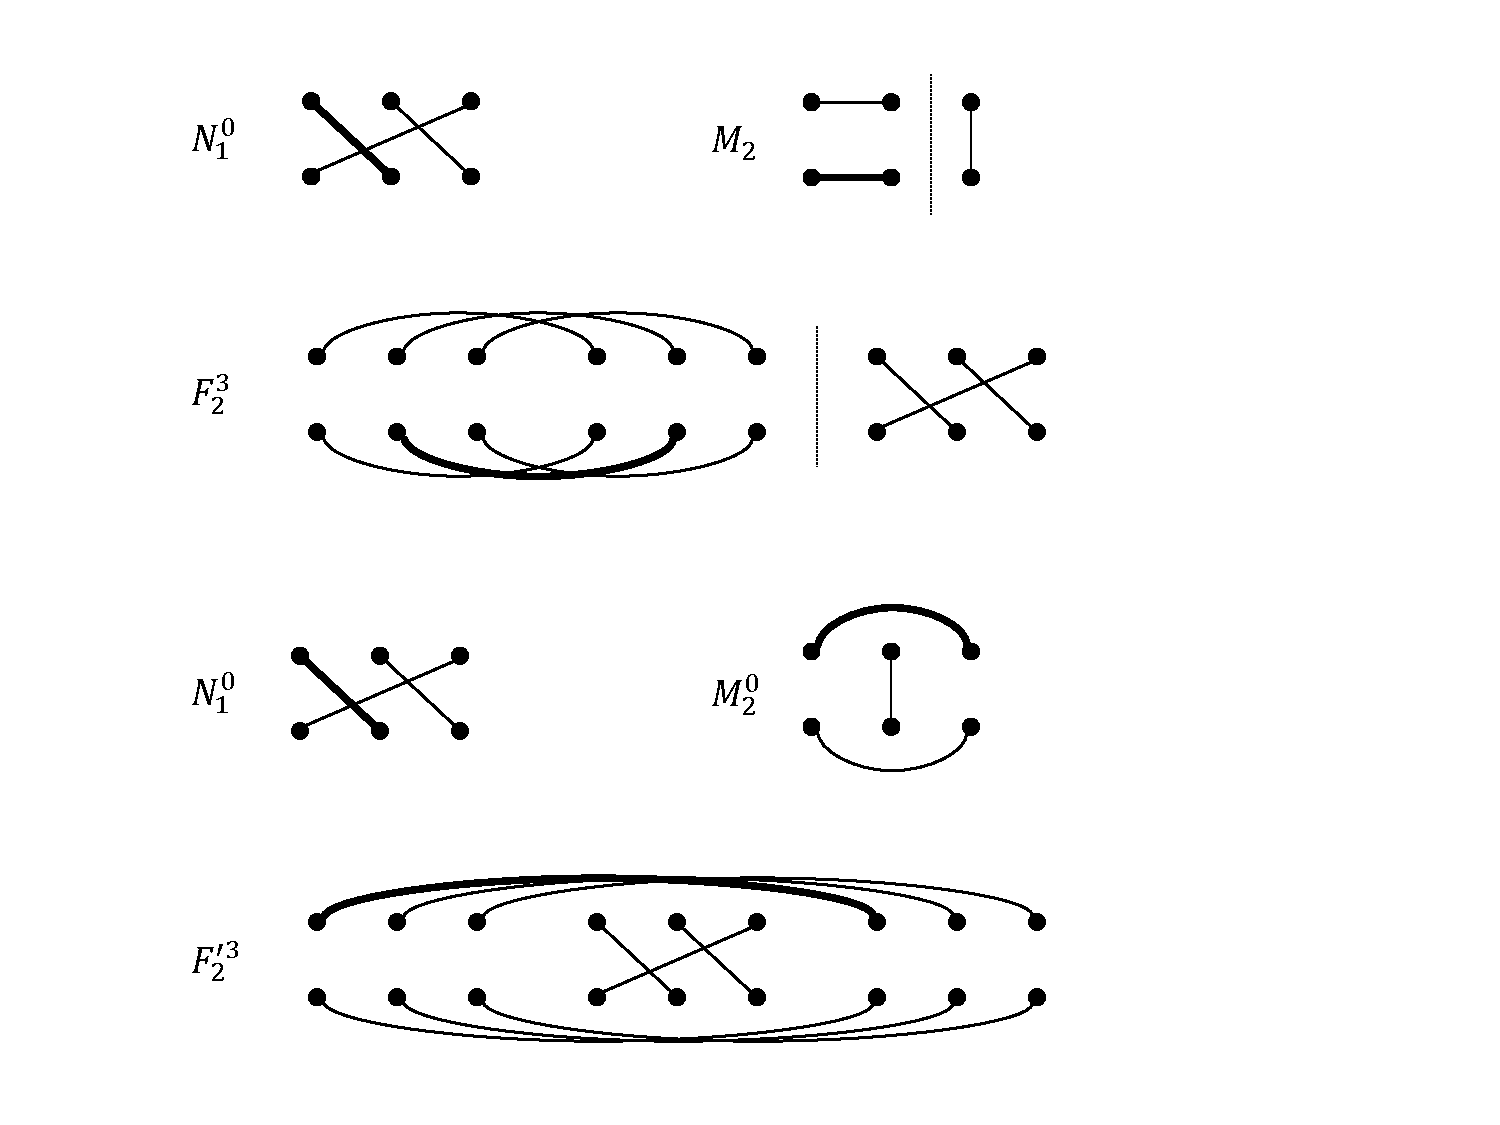
\includegraphics[width=0.39\textwidth]{figures/K_18-2.pdf}
\caption{$K_{18}$-ի որոշ կատարյալ զուգակցումներ հիմնված $K_6$-ի $\overline{\mathfrak{F}}=\{N_1,N_2,N_1^0,N_2^0,N_3^0\}$, $K_6$-ի $\widetilde{\mathfrak{F}}=\{M_1,M_2,M_1^0,M_2^0,M_3^0\}$ և $K_2\square K_6$-ի $\mathfrak{P}_6=\{P_0,P_1,P_2,P_3,P_4,P_5\}$ $1$-ֆակտորիզացիաների վրա՝ Լեմմա \ref{lComposite}-ի միջոցով:}
\label{K_18matchings}
\end{figure}


Ֆիքսենք, համապատասխանաբար, $K_{2mn}$-ի, $K_{2n}$-ի և $K_{2m}$-ի գագաթների համարակալումները.
\begin{align*}
\mathbf{v} &= \left(
u^1_1,v^1_1,u^1_2,v^1_2, \ldots, u^1_n,v^1_n,
u^2_1,v^2_1,u^2_2,v^2_2, \ldots, u^2_n,v^2_n, \ldots, 
u^m_1,v^m_1,u^m_2,v^m_2, \ldots, u^m_n,v^m_n \right) \\
\overline{\mathbf{v}} &= \left(
\overline{u}_1,\overline{v}_1,\overline{u}_2,\overline{v}_2, \ldots, \overline{u}_n,\overline{v}_n\right)\\
\widetilde{\mathbf{v}} &= \left(
\widetilde{u}^1,\widetilde{v}^1,\widetilde{u}^2,\widetilde{v}^2, \ldots, \widetilde{u}^m,\widetilde{v}^m\right)
\end{align*}

Դիցուք $\overline{\mathfrak{F}} = \{ N_1,N_2,\ldots,N_{\sigma_n},N^0_1,N^0_2,\ldots, N^0_{2n-1-\sigma_n} \}$ հանդիսանում է $K_{2n}$-ի $1$-ֆակտորիզացիա, որտեղ $N_i$-ն բաժանված կատարյալ զուգակցումներ է, երբ $i=1,2,\ldots,\sigma_n$: Դիցուք $\widetilde{\mathfrak{F}} = \{ M_1,M_2,\ldots,M_{\sigma_m},M^0_1,M^0_2,\ldots, M^0_{2m-1-\sigma_m} \}$ հանդիսանում է $K_{2m}$-ի $1$-ֆակտորիզացիա, որտեղ $M_i$-ն բաժանված կատարյալ զուգակցում է, երբ $i=1,2,\ldots,\sigma_m$: 

Մենք նաև կօգտագործենք $K_2 \square K_{2m}$ գրաֆը, $\left\{w_i,z_i : i=1,2,\ldots,2m\right\}$ գագաթների բազմությամբ, $\mathbf{w} = \left( w_1,z_1,w_2,z_2,\ldots,w_{2m},z_{2m} \right)$ գագաթների համարակալմամբ և իր $\mathfrak{P}_{2m} = \{P_0,P_1,\ldots,P_{2m-1} \}$ $1$-ֆակտորիզացիայով, որը սահմանվում է ինչպես այս պարագրաֆի սկզբում: $K_2 \square K_{2m}[\{w_{2k-1},w_{2k},z_{2k-1},z_{2k}\}]$ ենթագրաֆը կանվանենք $K_2 \square K_{2m}$-ի $k$-րդ բջիջ, որտեղ $1 \leq k \leq m$:

Ապացույցի ընթացքում միշտ կհամարենք, որ $x,y \in \{u,v\}$, $1 \leq s,t \leq n$ և $1 \leq p,q \leq m$:

Դիցուք $\overline{\varphi}$-ն արտապատկերում է $K_{2mn}$-ի կողերը $K_{2n}$-ի կողերի վրա: Ցանկացած $x^p_sy^q_t \in E(K_{2mn})$ կողի համար, որտեղ $x_s \neq y_t$, սահմանենք $\overline{\varphi}(x^p_sy^q_t)=\overline{x}_s\overline{y}_t$: Այնուհետև սահմանենք $\widetilde{\varphi}$ արտապատկերումը $K_{2mn}$-ի մնացած կողերից $K_{2m}$-ի կողերի մեջ: Ցանկացած $x^p_sx^q_s \in E(K_{2mn})$ կողի համար սահմանենք $\widetilde{\varphi}( x^p_sx^q_s ) = \widetilde{x}^p\widetilde{x}^q$: Նկատենք, որ $\overline{\varphi}^{-1}(\overline{e})$ նախապատկերները բոլոր $\overline{e} \in E(K_{2n})$ կողերի համար և $\widetilde{\varphi}^{-1}(\widetilde{x}^p\widetilde{x}^q)$ նախապատկերները բոլոր $\widetilde{x}^p\widetilde{x}^q \in E(K_{2m})$ կողերի համար զույգ առ զույգ տարբեր են, իսկ նրանց միավորումը ծածկում է ամբողջ $E(K_{2mn})$ բազմությունը: $E(K_{2mn})$ բազմությունը տրոհենք երեք չհատվող մասերի հետևյալ կերպ.
\begin{align*}
E(K_{2mn}) &= E^1 \cup E^2 \cup E^3 \text{, որտեղ} \\
E^1 &= \bigcup\limits_{i=1}^{\sigma_n}{\bigcup\limits_{\overline{e} \in N_i}{\overline{\varphi}^{-1}(\overline{e})}} \\
E^2 &= \bigcup\limits_{i=2}^{2n-1-\sigma_n}\bigcup\limits_{\overline{e} \in N^0_i}{\overline{\varphi}^{-1}(\overline{e})} \\
E^3 &= \bigcup\limits_{\overline{e} \in N^0_1}{\overline{\varphi}^{-1}(\overline{e})} \cup \bigcup\limits_{\widetilde{x}^p\widetilde{x}^q \in E(K_{2m})}{\widetilde{\varphi}^{-1}(\widetilde{x}^p\widetilde{x}^q)}
\end{align*}

$K_{2mn}$-ի կառուցվելիք $1$-ֆակտորիզացիան կնշանակենք $\mathfrak{F}$-ով և այն նույնպես բաղկացած կլինի երեք մասերից:

\begin{center}
$\mathfrak{F} = \mathfrak{F}^1 \cup \mathfrak{F}^2 \cup \mathfrak{F}^3$
\end{center}

$\mathfrak{F}^k$ կատարյալ զուգակցումների բազմությունը ծածկելու է $E^k$ կողերի բազմությունը, որտեղ $k=1,2,3$: Նկ. \ref{K_18matchings}-ում պատկերված են երեք մասերից յուրաքանչյուրը ծածկող կատարյալ զուգակցումները, երբ $m=n=3$:

$E^1$ բազմությունը բաղկացած է $K_{2n}$-ի բաժանված կատարյալ զուգակցումների նախապատկերներից: Այն ծածկելու համար կամայական $N_i \in \overline{\mathfrak{F}}$ բաժանված կատարյալ զուգակցման համար, $i=1,2,\ldots,\sigma_n$, և կամայական կենտ ինդեքսով $P_{2j+1} \in \mathfrak{P}_{2m}$ կատարյալ զուգակցման համար, $j=0,1,\ldots,m-1$, կառուցենք $\mathfrak{F}^1$-ի մեկ կատարյալ զուգակցում. 
\begin{align*}
F^1_{i,j} = &F^1_{i,j,1} \cup F^1_{i,j,2} \cup F^1_{i,j,3} \cup F^1_{i,j,4}\text{, որտեղ }\\
F^1_{i,j,1} = &\bigcup\limits_{\substack{w_{2k-1}z_{2k-1} \in P_{2j+1} \\ 1 \leq k \leq m}}
\left\{x_s^ky_t^k : \overline{x}_s\overline{y}_t \in l(N_i)\right\} \\
F^1_{i,j,2} = &\bigcup\limits_{\substack{w_{2k}z_{2k} \in P_{2j+1} \\ 1 \leq k \leq m}}
\left\{x_s^ky_t^k : \overline{x}_s\overline{y}_t \in r(N_i)\right\} \\
F^1_{i,j,3} = &\bigcup\limits_{\substack{w_{2k-1}w_{2l-1} \in P_{2j+1} \\ 1 \leq k < l \leq m}}
\left\{x_s^ky_t^l, y_t^kx_s^l : \overline{x}_s\overline{y}_t \in l(N_i)\right\} \\
F^1_{i,j,4} = &\bigcup\limits_{\substack{w_{2k}w_{2l} \in P_{2j+1} \\ 1 \leq k < l \leq m}}
\left\{x_s^ky_t^l, y_t^kx_s^l : \overline{x}_s\overline{y}_t \in r(N_i)\right\}\\
\mathfrak{F}^1 = &\left\{F^1_{i,j} : i=1,2,\ldots,\sigma_n,\ j=0,1,\ldots,m-1\right\}
\end{align*}

$F^1_{i,j,1}$-ը և $F^1_{i,j,2}$-ը կառուցելու համար դիտարկում ենք $P_{2j+1}$ կատարյալ զուգակցման ուղղաձիգ կողերը: Եթե որևէ $k$ թվի համար, $k$-րդ բջջի ձախ (աջ) կողմի ուղղաձիգ կողը պատկանում է $P_{2j+1}$-ին, ապա $K_{2mn}$-ի $k$-րդ $K_{2n}$-ի կրկնօրինակում $l(N_i)$-ի ($r(N_i)$-ի) բոլոր կողերի նախապատկերները ավելացնում ենք $F^1_{i,j,1}$-ին ($F^1_{i,j,2}$-ին): Ցանկացած $P_{2j+1}$ զուգակցում պարունակում է ճիշտ երկու ուղղաձիգ կող ($w_{j+1}z_{j+1}$ և $w_{j+m+1}z_{j+m+1}$): Երբ $m$-ը կենտ է, այդ երկու ուղղաձիգ կողերից մեկը գտնվում է իր բջջի ձախ մասում, իսկ մյուսը՝ իր բջջի աջ մասում: Երբ $m$-ը զույգ է, ապա եթե $j$-ն կենտ է (զույգ է), երկու ուղղաձիգ կողերն էլ գտնվում են իրենց բջիջների աջ (ձախ) կողմում: Այսպիսով, $F^1_{i,j,1}$-ի և $F^1_{i,j,2}$-ի կողերի քանակները կարելի է հաշվարկել հետևյալ կերպ.
\begin{align*}
|F^1_{i,j,1}| = &|l(N_i)|\left( (m \bmod 2)\cdot 1 + (1 - m \bmod 2)\cdot 2(1 - j \bmod 2) \right) \\
|F^1_{i,j,2}| = &|r(N_i)|\left( (m \bmod 2)\cdot 1 + (1 - m \bmod 2)\cdot 2(j \bmod 2) \right) 
\end{align*}

$F^1_{i,j,3}$-ը ($F^1_{i,j,4}$-ը) կառուցելու համար դիտարկում ենք $P_{2j+1}$-ի այն կողերը, որոնք միացնում են երկու տարբեր բջիջների ձախ (աջ) մասերը: Երբ $m$-ը կենտ է, գոյություն ունեն այդպիսի $\frac{m-1}{2}$ կողեր: Երբ $m$-ը զույգ է, ապա այդպիսի կողերի թիվը $\frac{m}{2} - (1 - j \bmod 2)$ է ($F^1_{i,j,4}$-ի դեպքում՝ $\frac{m}{2} - (j \bmod 2)$): $k$-րդ և $l$-րդ բջիջները ($k<l$) միացնող այդպիսի կողերից յուրաքանչյուրի համար $F^1_{i,j,3}$-ին ($F^1_{i,j,4}$-ին) ավելացնում ենք $l(N_i)$-ի ($r(N_i)$-ի) բոլոր այն նախապատկերները, որոնք միացնում են $K_{2mn}$-ում $K_{2n}$-ի $k$-րդ և $l$-րդ կրկնօրինակները: Նկատենք, որ $P_{2j+1}$-ի ամեն մի ֆիքսված կողին համապատասխանող $l(N_i)$-ի ($r(N_i)$-ի) յուրաքանչյուր կող ունի ճիշտ երկու նախապատկեր $F^1_{i,j,3}$-ում ($F^1_{i,j,4}$-ում). Ուստի ունենք հետևյալը.
\begin{align*}
|F^1_{i,j,3}| = &2|l(N_i)|\left( (m \bmod 2)\cdot \frac{m-1}{2} + (1 - m \bmod 2)\cdot \left(\frac{m}{2} - (1 - j \bmod 2)\right) \right) \\
|F^1_{i,j,4}| = &2|r(N_i)|\left( (m \bmod 2)\cdot \frac{m-1}{2} + (1 - m \bmod 2)\cdot \left(\frac{m}{2} - (j \bmod 2)\right) \right)
\end{align*}

$F^1_{i,j}$-ի կառուցումից հետևում է, որ այն զուգակցում է $K_{2mn}$-ում: Որպեսզի հիմնավորենք, որ այն նաև կատարյալ զուգացկում է, պետք է ցույց տալ, որ այն ունի ճիշտ $mn$ թվով կողեր: 
\begin{align*}
|F^1_{i,j}| = &|F^1_{i,j,1}| + |F^1_{i,j,2}| + |F^1_{i,j,3}| + |F^1_{i,j,4}| = \\
 = &|l(N_i)|\left(
 	(m \bmod 2)( 1 + m - 1) + 
    (1 - m \bmod 2)\left( 
    	2(1- j \bmod 2) + m - 2(1 - j\bmod 2) 
	\right)
\right) + \\
 + &|r(N_i)|\left(
 	(m \bmod 2)( 1 + m - 1) + 
    (1 - m \bmod 2)\left(
    	2(j \bmod 2) + m - 2(j\bmod 2)
    \right)
\right) \\
 = &\left(|l(N_i)| + |r(N_i)|\right)\left((m \bmod 2)\cdot m +  (1 - m \bmod 2)\cdot m \right) = nm
\end{align*}

$F^1_{i,j}$ և $F^1_{i',j'}$ զուգակցումները չեն հատվում, երբ $i \ne i'$ կամ $j \ne j'$, քանի որ նրանց կողերը համապատասխանում են կամ $K_{2n}$-ի տարբեր կողերի, կամ $K_2 \square K_{2m}$-ի տարբեր կողերի: Նաև նկատենք, որ եթե $N_i$-ն $r$-բաժանված կատարյալ զուգակցում է $\overline{\mathbf{v}}$ համարակալման նկատմամբ, ապա $F^1_{i,j}$-ը $(jn+r)$-բաժանված կատարյալ զուգակցում է $\mathbf{v}$ համարակալման նկատմամբ, բոլոր $i=1,2,\ldots,\sigma_n$ և $j=0,1,\ldots,m-1$ թվերի համար:

$E^2$ բազմությունը բաղկացած է բոլոր չբաժանված կատարյալ զուգակցումների նախապատկերներից, բացի մեկ չբաժանված կատարյալ զուգակցումից: Այն ծածկելու համար կամայական $N^0_i \in \overline{\mathfrak{F}}$ չբաժանված կատարյալ զուգակցման համար, բացի $N^0_1$-ից (այս բացառության ընտրությունը կամայական է) և կամայական զույգ ինդեքսով $P_{2j} \in \mathfrak{P}_{2m}$ կատարյալ զուգակցման համար կառուցենք $\mathfrak{F}^2$-ի մեկ կատարյալ զուգակցում:
\begin{align*}
F^2_{i,j} = &F^2_{i,j,1} \cup F^2_{i,j,2}\text{, որտեղ }\\
F^2_{i,j,1} = &\bigcup\limits_{\substack{w_{2k-1}w_{2k} \in P_{2j} \\ 1 \leq k \leq m}}
\left\{x_s^ky_t^k : \overline{x}_s\overline{y}_t \in N^0_i\right\} \\
F^2_{i,j,2} = &\bigcup\limits_{\substack{w_{2k-1}w_{2l} \in P_{2j} \\ 1 \leq k < l \leq m}}
\left\{x_s^ky_t^l, y_t^kx_s^l : \overline{x}_s\overline{y}_t \in N^0_i\right\}\\
\mathfrak{F}^2 = &\{F^2_{i,j} : i=2,3,\ldots,2n-1-\sigma_n,\ j=0,1,\ldots,m-1\}
\end{align*}
$P_{2j}$ զուգակցումները ունեն միայն հորիզոնական կողեր: Մեզ հետաքրքրում են այն կողերը, որոնք միացնում են որևէ բջջի ձախ մասը որևէ բջջի (նույն կամ տարբեր) աջ մասի հետ: Եթե կողի երկու ծայրակետերն էլ պատկանում են միևնույն $k$-րդ բջջին, ապա $N_i^0$-ի բոլոր կողերի այն նախապատկերները, որոնք $K_{2mn}$-ում պատկանում են $K_{2n}$-ի $k$-րդ կրկնօրինակին, ավելացնում ենք $F^2_{i,j,1}$ բազմությանը: $P_{2j}$-ում այդպիսի կողերի քանակը $1$ է, եթե $m$-ը կենտ է, և $2(j \bmod 2)$ է, եթե $m$-ը զույգ է: Ուստի, ունենք.
\begin{align*}
|F^2_{i,j,1}| = &n\left( (m \bmod 2)\cdot 1 + (1 - m \bmod 2)\cdot 2(j \bmod 2) \right)
\end{align*}
Եթե $P_{2j}$-ի կողը միացնում է $k$-րդ և $l$-րդ բջիջները ($k < l$), ապա $N_i^0$-ի բոլոր կողերի այն նախապատկերները, որոնք միացնում են $K_{2mn}$-ում $K_{2n}$-ի $k$-րդ և $l$-րդ կրկնօրինակների գագաթները, ավելացնում ենք $F^2_{i,j,2}$ բազմությանը: $P_{2j}$-ում այդպիսի կողերի քանակը $\frac{m-1}{2}$ է, եթե $m$-ը կենտ է, և $\frac{m}{2} - (j \bmod 2)$ է, եթե $m$-ը զույգ է: Ուստի.
\begin{align*}
|F^2_{i,j,2}| = &2n\left( (m \bmod 2)\cdot \frac{m-1}{2} + (1 - m \bmod 2)\cdot \left(\frac{m}{2} - (j \bmod 2)\right) \right) \\
|F^2_{i,j}| = &|F^2_{i,j,1}| + |F^2_{i,j,2}| =\\
= &n\left(
	(m \bmod 2)(1+m-1) + 
    (1 - m \bmod 2)(2(j \bmod 2) + m - 2(j \bmod 2))
\right) =\\
= &n\left(
	(m \bmod 2) \cdot m + 
    (1 - m \bmod 2) \cdot m
\right) = nm
\end{align*}

Ինչպես $\mathfrak{F}^1$-ի զուգակցումների դեպքում, $F^2_{i,j}$ և $F^2_{i',j'}$ զուգակցումները նույնպես չեն հատվում, երբ $i \ne i'$ կամ $j \ne j'$: Նկատենք, որ կամայական $i=2,3,\ldots,2n-1-\sigma_n$ թվի համար, $F^2_{i,j}$-ն $jn$-բաժանված կատարյալ զուգակցում է $\mathbf{v}$ համարակալման նկատմամբ երբ $j=1,2,\ldots,m-1$, իսկ երբ $j=0$, այն բաժանված կատարյալ զուգակցում չէ:

$E^3$ բազմությունը պարունակում է $K_{2n}$-ի $N^0_1$ չբաժանված կատարյալ զուգակցման բոլոր կողերի նախապատկերները և $K_{2m}[\{\widetilde{u}^1,\widetilde{u}^2,\ldots,\widetilde{u}^m\}] \cup K_{2m}[\{\widetilde{v}^1,\widetilde{v}^2,\ldots,\widetilde{v}^m\}]$ ենթագրաֆի բոլոր կողերի նախապատկերները: $K_{2m}$-ի կողերի նախապատկերները կազմում են թվով $2n$ իրար հետ չհատվող, $m$ գագաթանի լրիվ գրաֆներ՝ $K_{2mn}\left[\{x_s^1,x_s^2,\ldots,x_s^m\}\right]$, կամայական $\overline{x}_s \in V(K_{2n})$ գագաթի համար: Կամայական $\overline{x}_s\overline{y}_t \in N^0_1$ կողի համար, իր նախապատկերը և իր երկու $\overline{x}_s$ և $\overline{y}_t$ ծայրակետերին համապատասխանող $K_{m}$ ենթագրաֆները կազմում են $K_{2mn}\left[\{x_s^1,y_t^1,x_s^2,y_t^2,\ldots,x_s^m,y_t^m\}\right]$ ենթագրաֆը, որը իզոմորֆ է $K_{2m}$-ին: Այսինքն, $E^3$ բազմությունը կազմված է $K_{2m}$-ի թվով $n$ չհատվող կրկնօրինակներից: Կամայական $M \in \widetilde{\mathfrak{F}}$ կատարյալ զուգակցման համար կառուցում ենք $K_{2mn}$-ում մեկ կատարյալ զուգակցում միավորելով $E^3$-ում իր $n$ չհատվող կրկնօրինակները: 
\begin{align*}
F^3_{i} = &
\bigcup\limits_{\substack{\overline{x}_s\overline{y}_t \in N^0_1}}
\left\{ 
\{x_s^{p}x_s^{q} : \widetilde{u}^{p}\widetilde{u}^{q} \in M_i\} 
\cup 
\{x_s^{p}y_t^{q} : \widetilde{u}^{p}\widetilde{v}^{q} \in M_i\} 
\cup
\{y_t^{p}y_t^{q} : \widetilde{v}^{p}\widetilde{v}^{q} \in M_i\} 
\right\}\\
F'^3_{i} = &
\bigcup\limits_{\substack{\overline{x}_s\overline{y}_t \in N^0_1}}
\left\{ 
\{x_s^{p}x_s^{q} : \widetilde{u}^{p}\widetilde{u}^{q} \in M^0_i\} 
\cup 
\{x_s^{p}y_t^{q} : \widetilde{u}^{p}\widetilde{v}^{q} \in M^0_i\} 
\cup
\{y_t^{p}y_t^{q} : \widetilde{v}^{p}\widetilde{v}^{q} \in M^0_i\} 
\right\}\\
\mathfrak{F}^3 = &\left\{F^3_{i} : i=1,2,\ldots,\sigma_m\right\} \cup \left\{F'^3_{i} : i=1,2,\ldots,2m-1-\sigma_m\right\}
\end{align*}
$F^3_i$ և $F'^3_i$ զուգակցումները զույգ առ զույգ չեն հատվում և յուրաքանչյուրը բաղկացած է $mn$ կողերից: Նկատենք, որ եթե $M_i$-ն $r$-բաժանված կատարյալ զուգակցում է $\widetilde{\mathbf{v}}$ համարակալման նկատմամբ, ապա $F^3_i$-ն, $i=1,2,\ldots,\sigma_m$, $rn$-բաժանված կատարյալ զուգակցում է $\mathbf{v}$ համարակալման նկատմամբ: Իսկ $F'^3_i$, $i=1,2,\ldots,2m-1-\sigma_m$, կատարյալ զուգակցումները բաժանված չեն:

$\mathfrak{F}$ բազմության մեջ կատարյալ զուգակցումների թիվը $m\sigma_n + m(2n-2-\sigma_n) + 2m-1 = 2mn-1$ է: Այս կատարյալ զուգակցումներից բաժանված են միայն $m\sigma_n + (m-1)(2n-2-\sigma_n) + \sigma_m = \sigma_m+\sigma_n+2(m-1)(n-1)$ հատը: Ապացույցն ավարտված է:
\end{proof}

Կիրառելով Համարժեքության թեորեմը ստանում ենք հետևյալ ստորին գնահատականը, որն ընդհանրացնում է Թեորեմ \ref{tPetrosyan4n}-ը.
\begin{theorem}
\label{tComposite}
Ցանկացած $m,n \in\mathbb{N}$ թվերի համար $W(K_{2mn}) \geq W(K_{2m}) + W(K_{2n}) + 4(m-1)(n-1) - 1$:
\end{theorem}

Հայտնի է, որ $W(K_6) = 7$ և $W(K_{10}) \geq 14$: Վերոնշյալ թեորեմից հետևում է, որ $W(K_{30}) \geq 52$, ինչը հերքում է Հիպոթեզ \ref{h1_complete_log}-ը, ըստ որի $W(K_{30})=51$: Ինչպես կտեսնենք այս պարագրաֆի վերջում, սա հիպոթեզը հերքող ամենափոքր օրինակը չէ:

\begin{theorem}
\label{t1_lower}
Եթե $n=\prod\limits_{i=1}^{\pi(n)}p_i^{\alpha_i}$, որտեղ $p_i$-ն $i$-րդ պարզ թիվն է, $\pi(n)$-ը՝ $n$-ը չգերազանցող պարզ թվերի քանակը, իսկ $\alpha_i \in \mathbb{Z}_{\geq 0}$, ապա
\begin{center}
$W(K_{2n}) \geq 4n - 3 - \sum\limits_{i=1}^{\pi(n)}{\alpha_i\left(4p_i-3-W(K_{2p_i})\right)}$:
\end{center}
\end{theorem}
\begin{proof}[Ապացույց]
$d_m$-ով նշանակենք $W(K_{2m}) - (4m - 3)$ տարբերությունը: Թեորեմ \ref{tComposite}-ը պնդում է, որ $d_{mk} \geq d_m + d_k$: Մաթեմատիկական ինդուկցիայի եղանակով ստանում ենք, որ $d_n \geq \sum_{i=1}^{\pi(n)}{\alpha_i d_{p_i}}$: Ապացույցը կավարտվի, եթե $d_{p_i}$-ի փոխարեն տեղադրենք իր արժեքը:
\end{proof}

Մինչև $W(K_{2n})$-ի վերին գնահատականներին անցնելը ցույց տանք, որ վերը շարադրված թեորեմները թույլ են տալիս գնահատել նաև $W(G)$ պարամետրը, երբ $G$-ն ստացվում է լրիվ գրաֆից մեկ կատարյալ զուգակցում հանելով:

\begin{theorem}
\label{t1-complete-minus-matching}
Եթե $G$ գրաֆը ստացվում է $K_{2n}$ լրիվ գրաֆից մեկ կատարյալ զուգակցում հանելով, ապա $W(G) \geq W(K_{2n})-1$:
\end{theorem}
\begin{proof}[Ապացույց]
Դիցուք $\alpha$-ն $K_{2n}$-ի որևէ միջակայքային $W(G)$-ներկում է, որի համար ${\rm sh}(\alpha) = (b_1, b_2, \ldots b_{n-1})$: Ըստ Պնդում \ref{spectrumIntersection}-ի $K_{2n}$-ում գոյություն ունի $F$ կատարյալ զուգակցում, որի բոլոր կողերը ներկված են միևնույն $c$ գույնով: $K_{2n}$ գրաֆից հանենք $F$ զուգակցումը և ստացված գրաֆի համար կառուցենք $\beta$ ներկումը հետևյալ կերպ.
\begin{align*}
    \beta(e) &= \left\{
\begin{tabular}{ll}
$\alpha(e)$, & երբ $\alpha(e) < c$\\
$\alpha(e) - 1$, & երբ $\alpha(e) > c$
\end{tabular}%
\right.
\end{align*}
Կամայական $v \in V(K_{2n}-F)$ գագաթի սպեկտրը կլինի $S(v,\beta) = \left[\underline{S}(v,\alpha), \overline{S}(v,\alpha)-1\right]$: Հետևաբար, $\beta$-ն $K_{2n}-F$ գրաֆի միջակայքային $\left(W(K_{2n})-1\right)$-ներկում է և $W(K_{2n} - F) \geq W(K_{2n})-1$: 
\end{proof}



\subsubsection{Վերին գնահատականներ}


\begin{figure}[t!]
\centering
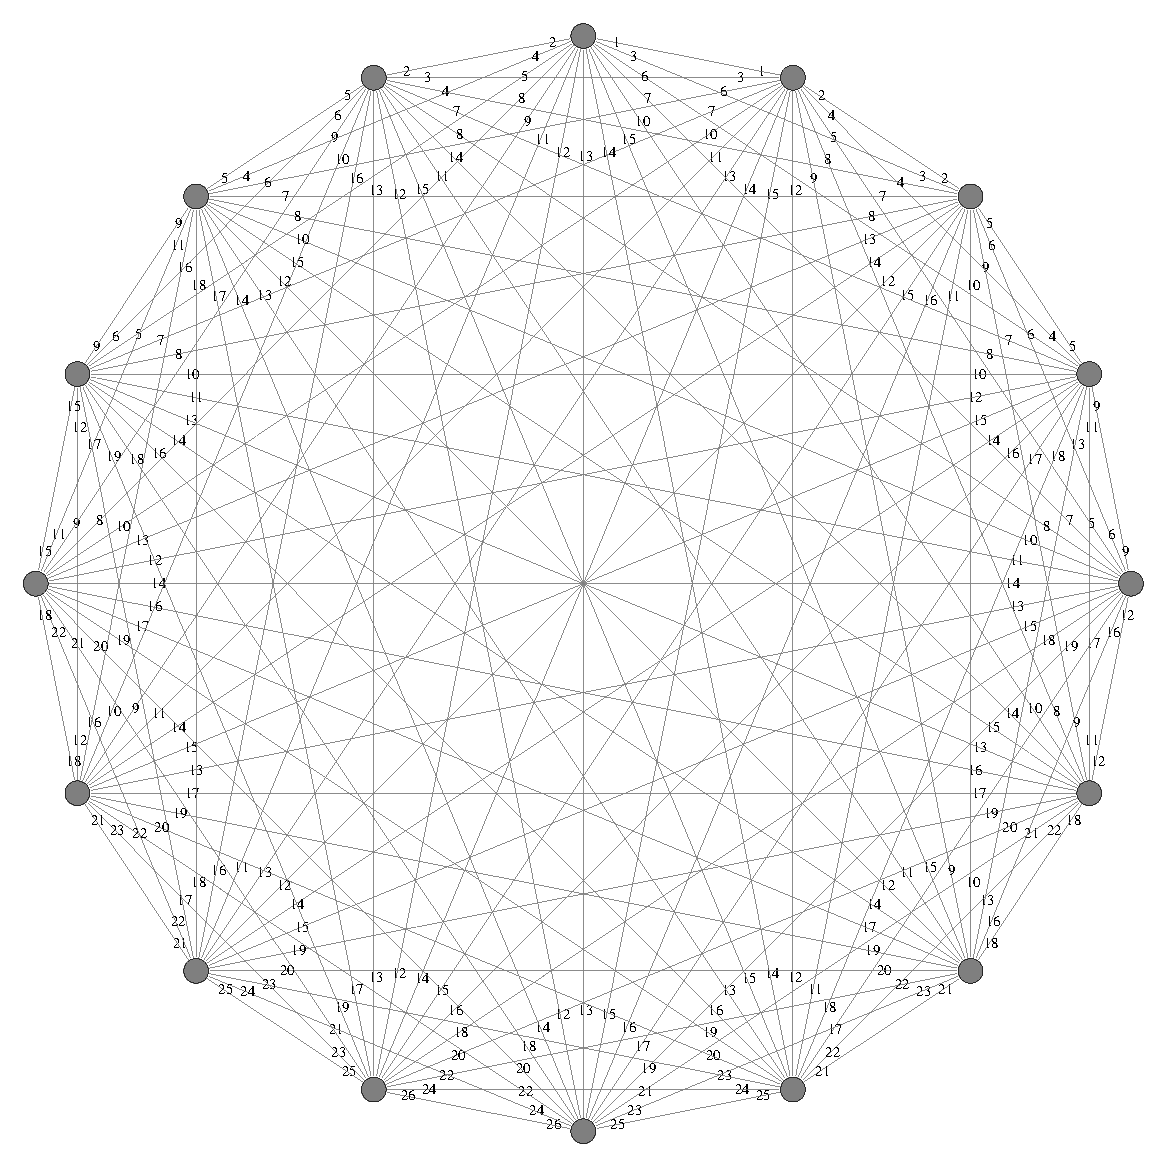
\includegraphics[width=\textwidth]{figures/K_16-26.pdf}
\caption{$K_{16}$-ի միջակայքային $26$-ներկում: ${\rm sh}(\alpha) = (1,2,1,3,1,2,1)$}
\label{f2_K16}
\end{figure}



Դիցուք $\alpha$-ն $K_{2n}$-ի կամայական միջակայքային կողային ներկում է, $n \in \mathbb{N}$, իսկ $\mathbf{v}_\alpha = \left(u_1,v_1, u_2,v_2, \ldots,u_n,v_n\right)$ ներկմանը համապատասխանող գագաթների համարակալումն է: Դիցուք $\alpha$-ի շեղման վեկտորն է ${\rm sh}(\alpha) = (b_1,b_2,\ldots,b_{n-1})$: Համարժեքության լեմմայից հետևում է, որ գոյություն ունի $K_{2n}$-ի $\mathfrak{F} = 
\left\{ F^0_j : j=1,2,\ldots,2n-1-\sum\limits_{i=1}^{n-1}b_i \right\}
\cup
\bigcup\limits_{i=1}^{n-1}\left\{F^i_j : j=1,2,\ldots,b_i\right\}$ 1-ֆակտորիզացիա այնպես, որ $F^i_j$-ն $i$-բաժանված է $\mathbf{v_\alpha}$ համարակալման նկատմամբ, $i=1,2,\ldots,n-1$, $j=1,2,\ldots,b_i$: Այս բաժնի բոլոր այն ապացույցներում, որտեղ կունենանք լրիվ գրաֆի $\alpha$ միջակայքային ներկում, կենթադրենք, որ տրված է նաև գագաթների համապատասխան $\mathbf{v}_{\alpha}$ համարակալումը և $\mathfrak{F}$ 1-ֆակտորիզացիան:

$W(K_{2n})$-ի վերին գնահատականները լավացնելու համար մեզ պետք կգան մի շարք լեմմաներ:

\begin{lemma}
\label{lReverse}
Եթե $K_{2n}$-ի որ և $\alpha$ միջակայքային կողային ներկման շեղման վեկտորը ${\rm sh}(\alpha) = (b_1,b_2,\ldots, b_{n-1})$ է, ապա գոյություն ունի $K_{2n}$-ի $\beta$ միջակայքային կողային ներկում այնպես, որ ${\rm sh}(\beta) = (b_{n-1}, b_{n-2}, \ldots, b_1)$:
\end{lemma}
\begin{proof}[Ապացույց]
Նկատենք, որ եթե որևէ $F \in \mathfrak{F}$ $i$-բաժանված է $\mathbf{v}_\alpha$ համարակալման նկատմամբ, ապա այն կլինի $(n-i)$-բաժանված $\mathbf{v}'_\alpha = \left(u_n,v_n,u_{n-1},v_{n-1},\ldots,u_1,v_1\right)$ համարակալման նկատմամբ: 
Կիրառենք Համարժեքության լեմման $\mathfrak{F}$-ից $\mathbf{v}'_\alpha$ համարակալման նկատմամբ $\beta$ ներկումը կառուցելու համար: Շեղումների վեկտորը կլինի $(b_{n-1}, b_{n-2}, \ldots, b_1)$:
\end{proof}

\begin{lemma}
\label{lLessColors}
Եթե $K_{2n}$-ի որևէ $\alpha$ միջակայքային կողային ներկման համար ${\rm sh}(\alpha) = (b_1,b_2,\ldots, b_{n-1})$, որտեղ $b_i > 0$ որևէ $i \in [1,n-1]$ թվի համար, ապա գոյություն ունի $K_{2n}$-ի $\beta$ միջակայքային կողային ներկում այնպես, որ ${\rm sh}(\beta) = (b_1, b_2, \ldots, b_{i-1}, b_{i}-1, b_{i+1}, \ldots, b_{n-1})$:
\end{lemma}
\begin{proof}[Ապացույց]
$b_i > 0$ պայմանից հետևում է, որ գոյություն ունի $F_{b_i}^i \in \mathfrak{F}$ կատարյալ զուգակցում, որը $i$-բաժանված է $\mathbf{v}_\alpha$ համարակալման նկատմամբ: Կառուցենք $\beta$ ներկումը կիրառելով Համարժեքության լեմման $\mathfrak{F}$ 1-ֆակտորիզացիայի նկատմամբ, համարելով $F_{b_i}^i$ զուգակցումը չբաժանված (կարող ենք վերանվանել այն $F^0_{2n-|{\rm sh}(\alpha)|}$):
\end{proof}


\begin{lemma}
\label{l2k1}
Եթե $K_{2n}$-ի որևէ $\alpha$ միջակայքային կողային ներկման համար ${\rm sh}(\alpha) = (b_1,b_2,\ldots, b_{n-1})$, ապա
\begin{center}
$\sum\limits_{i=1}^{k}{b_i} \leq 2k-1$, որտեղ $k=1,2,\ldots,n-1$:
\end{center}
\end{lemma}

\begin{proof}[Ապացույց]
Համարժեքության լեմմայի ապացույցի համաձայն $F^i_j$ կատարյալ զուգակցումների ձախ մասերը ծածկում են $u_1$ գագաթը (ինչպես նաև $v_1$-ը), $i=1,2,\ldots,k$, $j=1,2,\ldots,b_i$: Ավելին, 
\begin{center}
$\bigcup\limits_{i=1}^{k}
\bigcup\limits_{j=1}^{b_i}
{l^i_{\mathbf{v}_\alpha}\left(F^i_j\right)} 
\subset E\left(H_{\mathbf{v}_\alpha}^{[1,k]}\right)$
\end{center}
Ապացույցն ավարտելու համար նկատենք, որ $F^i_j$ կատարյալ զուգակցումների քանակը $\sum\limits_{i=1}^{k}{b_i}$ է, իսկ $u_1$ (կամ $v_1$) գագաթի աստիճանը $H_{\mathbf{v}_\alpha}^{[1,k]}$ ենթագրաֆում $2k-1$ է:
\end{proof}

$(b_1,b_2,\ldots,b_k)$ վեկտորը կանվանենք \textit{հագեցած}, եթե $\sum\limits_{i=1}^{k}{b_i} = 2k-1$:

\begin{corollary}
\label{c2n4}
Եթե $\alpha$-ն $K_{2n}$-ի միջակայքային կողային ներկում է, $n\geq 3$, ապա  
$|{\rm sh}(\alpha)| \leq 2n-4$:
\end{corollary}

\begin{proof}[Ապացույց]
Դիցուք ${\rm sh}(\alpha) = (b_1,b_2,\ldots, b_{n-1})$: Լեմմա \ref{l2k1}-ից հետևում է, որ $\sum\limits_{i=1}^{n-2}{b_i} \leq 2n-5$: Նույն լեմմայից Լեմմա \ref{lReverse}-ի հետ համատեղ բխում է, որ $b_{n-1} \leq 1$: Ապացույցը կավարտենք գումարելով այս երկու անհավասարությունները:
\end{proof}

\begin{lemma}
\label{lAfterSaturated}
Եթե $K_{2n}$-ի որևԷ $\alpha$ միջակայքային կողային ներկման համար ${\rm sh}(\alpha) = (b_1,b_2,\ldots, b_{n-1})$, և $(b_1,b_2,\ldots,b_k)$ վեկտորը հագեցած է որևէ $k \in [2,n-2]$ թվի համար, ապա $b_{k+1} \leq 1$:
\end{lemma}

\begin{proof}[Ապացույց]
Լեմմա \ref{l2k1}-ից հետևում է, որ $b_{k+1} \leq 2$: Ապացույցն ավարտելու համար անհրաժեշտ է ցույց տալ, որ $b_{k+1} \neq 2$: Ենթադրենք հակառակը՝ $b_{k+1} = 2$: $(b_1,b_2,\ldots,b_k)$ վեկտորը հագեցած է, ուստի Լեմմա \ref{l2k1}-ի ապացույցից բխում է, որ $u_1x_i$ և $v_1x_i$ կողերը, $x \in \{u,v\}$, $i=2,3,\ldots,k$, պատկանում են $F^i_j$ կատարյալ զուգակցումներին, $i=1,2,\ldots,k$, $j=1,2,\ldots,b_i$: Նմանապես, $u_1u_{k+1}$, $u_1v_{k+1}$, $v_1u_{k+1}$ և $v_1v_{k+1}$ կողերը պետք է ծածկված լինեն $F^{k+1}_1$-ով և $F^{k+1}_2$-ով:

Այժմ դիտարկենք $u_2$ գագաթը: Այն ծածկված է $F^i_j$ կատարյալ զուգակցումների ձախ մասերով, $i=2,3,\ldots,k$, $j=1,2,\ldots,b_i$: Բոլոր այս զուգակցումները միասին ծածկում են $H_{\mathbf{v}_\alpha}^{[1,k]}$ ենթագրաֆում $u_2$-ին կից բոլոր կողերը, բացի $2k-1 - \sum\limits_{i=2}^{k}{b_i} = b_1$ կողերից: Լեմմա \ref{l2k1}-ից բխում է, որ $b_1 \leq 1$, ուստի չծածկված մնում է առավելագույնը մեկ կող: $u_2$ գագաթը պետք է ծածկված լինի նաև $F^{k+1}_1$ և $F^{k+1}_2$ կատարյալ զուգակցումների ձախ մասերով: $u_2u_{k+1}$ և $u_2v_{k+1}$ կողերը չեն կարող օգտագործվել, քանի որ $u_{k+1}$ և $v_{k+1}$ արդեն ծածկված են $F^{k+1}_1$-ով և $F^{k+1}_2$-ով: Հետևաբար, այս երկու զուգակցումների մնում է առավելագույնը մեկ կող, ինչը հակասություն է:
\end{proof}


\begin{corollary}
\label{c2n5}
Եթե $\alpha$-ն $K_{2n}$-ի միջակայքային ներկում է և $n\geq 5$, ապա  
$|{\rm sh}(\alpha)| \leq 2n-5$:
\end{corollary}

\begin{proof}[Ապացույց]
Դիցուք ${\rm sh}(\alpha) = (b_1,b_2,\ldots, b_{n-1})$: Լեմմա \ref{l2k1}-ից հետևում է, որ $\sum\limits_{i=1}^{n-3}{b_i} \leq 2n-7$: Դիտարկենք երկու դեպք.
\begin{description}
\item{Դեպք 1.} $\sum\limits_{i=1}^{n-3}{b_i} = 2n-7$: Լեմմա \ref{lAfterSaturated}-ից բխում է, որ $b_{n-2} \leq 1$: Լեմմաներ \ref{lReverse} և \ref{l2k1}-ից հետևում է, որ $b_{n-1} \leq 1$: Գումարելով այս անհավասարությունները կստանանք պահանջված գնահատականը:
\item{Դեպք 2.} $\sum\limits_{i=1}^{n-3}{b_i} \leq 2n-8$: Լեմմաներ \ref{lReverse}-ից և \ref{l2k1}-ից հետևում է, որ $b_{n-2} + b_{n-1} \leq 3$: Գումարելով այս անհասավարությունները կավարտենք ապացույցը:
\end{description}
\end{proof}


\begin{lemma}
\label{lBeforeSaturated}
Եթե $K_{2n}$-ի որևէ $\alpha$ միջակայքային կողային ներկման համար ${\rm sh}(\alpha) = (b_1,b_2,\ldots, b_{n-1})$, և $(b_1,b_2,\ldots,b_k)$ վեկտորը հագեցած է որևէ $k \in [3,n-1]$ թվի համար, ապա $b_{k} \geq 3$:
\end{lemma}

\begin{proof}[Ապացույց]
Ենթադրենք հակառակը՝ $b_k \leq 2$: Եթե $b_k=2$, ապա $(b_1,b_2,\ldots,b_{k-1})$ վեկտորը ևս հագեցած է, ինչը բերում է հակասության Լեմմա \ref{lAfterSaturated}-ի հետ: Եթե $b_k \leq 1$, ապա ունենք, որ $\sum\limits_{i=1}^{k-1}{b_i} \geq 2k-2$, ինչը հակասում է Լեմմա \ref{l2k1}-ին:
\end{proof}



\begin{lemma}
\label{lEdgeCount}
Եթե $K_{2n}$-ի որևէ $\alpha$ միջակայքային կողային ներկման համար ${\rm sh}(\alpha) = (b_1,b_2,\ldots, b_{n-1})$, և $k \in [2,n-2]$, ապա
\begin{center}
$k(2k-1) \geq \sum\limits_{i=1}^{k}{ib_i} + \sum\limits_{i=k+1}^{\min\{2k-1,n-1\}}{(2k-i)b_i}$:
\end{center}
\end{lemma}
\begin{proof}[Ապացույց]
Դիտարկենք $H_{\mathbf{v}_\alpha}^{[1,k]}$ ենթագրաֆը: Այս ենթագրաֆում կողերի քանակը $k(2k-1)$ է: $F^i_j$ կատարյալ զուգակցումներից յուրաքանչյուրի ձախ մասը, $i=1,2,\ldots,k$, $j=1,2,\ldots,b_i$, բաղկացած է $i$ կողերից, և բոլորն էլ պատկանում են $H_{\mathbf{v}_\alpha}^{[1,k]}$ ենթագրաֆին: Այսպիսի կողերի քանակն է $\sum\limits_{i=1}^{k}{ib_i}$:

Այժմ ֆիքսենք որևէ $i \in [k+1,r]$, որտեղ $r$-ով նշանակել ենք $\min\{2k-1,n-1\}$-ը: $F_j^i$ կատարյալ զուգակցումներից յուրաքանչյուրի ձախ մասը, $j=1,2,\ldots,b_i$, բաղկացած է $i$ կողերից: Դրանցից առավելագույնը $(2i-2k)$-ը կարող են միացնել $H_{\mathbf{v}_\alpha}^{[1,k]}$-ի որևէ գագաթ $H_{\mathbf{v}_\alpha}^{[k+1,i]}$-ի որևէ գագաթի հետ: Ուստի առնվազն $2k-i$ կողեր պատկանում են $H_{\mathbf{v}_\alpha}^{[1,k]}$ ենթագրաֆին: Այդպիսի կողերի քանակը առնվազն $\sum\limits_{i=k+1}^{r}{(2k-i)b_i}$ է:
\end{proof}

Լեմմա \ref{lEdgeCount}-ից հետևում է, որ եթե որևէ ֆիքսված $k_0$-ի համար գոյություն ունեն մեծ թվով $i$-բաժանված կատարյալ զուգակցումներ, որտեղ $i \leq k_0$, ապա չեն կարող գոյություն ունենալ մեծ թվով $i'$-բաժանված կատարյալ զուգակցումներ, որտեղ $k_0 < i' < \min\{2k_0-1,n-1\}$: Այս լեմման օգտագործելու համար հարկավոր է $\sum\limits_{i=1}^{k}{ib_i}$ գումարը գնահատել ներքևից:

Կամայական $k\in \mathbb{N}$ և $r \in \mathbb{Z}_{\geq 0}$ թվերի համար սահմանենք հետևյալը.
\begin{align*}
&T_k = \left\{\left(b_1,b_2,\ldots,b_k\right) : \exists K_{2n}\text{-ի }\alpha \text{միջակայքային ներկում},\ n>k,\ {\rm sh}(\alpha)=(b_1,b_2,\ldots,b_{n-1})\right\} \\
&m(k,r) = \min\limits_{(b_1,b_2,\ldots,b_{k}) \in T_k}\left\{\sum\limits_{i=1}^{k}{ib_i} : \sum\limits_{i=1}^{k}{b_i}=r\right\}
\end{align*}
Նկատենք, որ $m(k,r)$-ը սահմանված չէ բոլոր $(k,r)$ զույգերի համար: Օրինակ, Լեմմա \ref{l2k1}-ից հետևում է, որ գոյություն չունեն $K_{2n}$-ի այնպիսի միջակայքային ներկումներ, որոնց համար $\sum\limits_{i=1}^{k}{b_i}=r$, երբ $r \geq 2k$: Ակնհայտ է, որ $m(1,1)=1$ և $m(k,0)=0$, որտեղ $k \in \mathbb{N}$:

\begin{remark}
$m(k,r)$-ը հաշվելու համար, $k>1$, $r>1$, բավական է վերցնել մինիմումը ըստ բոլոր այն $(b_1,b_2,\ldots,b_k) \in T_k$ վեկտորների, որոնց համար $\sum\limits_{i=1}^{k-1}{ib_i} = m(k-1,r-b_k)$:
\end{remark}


\begin{table}[t!]
\centering
\newcolumntype{C}{>{\centering\arraybackslash}X}%

\begin{tabularx}{0.8\textwidth}{c||C|C|C|C|}
\backslashbox{$r$}{$k$} & $1$ & $2$ & $3$ & $4$ \\ \hline\hline
$0$
& \begin{tabular}{c}$0$ \\ $(0)$ \end{tabular} 
& \begin{tabular}{c}$0$ \\ $(0,0)$ \end{tabular} 
& \begin{tabular}{c}$0$ \\ $(0,0,0)$ \end{tabular}  
& \begin{tabular}{c}$0$ \\ $(0,0,0,0)$ \end{tabular} \\ \hline

$1$ 
& \begin{tabular}{c}$1$ \\ $(1)$ \end{tabular} 
& \begin{tabular}{c}$1$ \\ $(1,0)$ \end{tabular} 
& \begin{tabular}{c}$1$ \\ $(1,0,0)$ \end{tabular} 
& \begin{tabular}{c}$1$ \\ $(1,0,0,0)$ \end{tabular} \\ \hline

$2$
&
& \begin{tabular}{c}$3$ \\ $(1,1)$ \end{tabular}  
& \begin{tabular}{c}$3$ \\ $(1,1,0)$ \end{tabular}  
& \begin{tabular}{c}$3$ \\ $(1,1,0,0)$ \end{tabular} \\ \hline

$3$
&
& \begin{tabular}{c}$5$ \\ $(1,2)$ \end{tabular}  
& \begin{tabular}{c}$5$ \\ $(1,2,0)$ \end{tabular} 
& \begin{tabular}{c}$5$ \\ $(1,2,0,0)$ \end{tabular} \\ \hline 


$4$
&
&
& \begin{tabular}{c}$8$ \\ $(1,2,1)$ \end{tabular} 
& \begin{tabular}{c}$8$ \\ $(1,2,1,0)$ \end{tabular} \\ \hline

$5$
&
&
& \begin{tabular}{c}$12$ \\ $(1,1,3)$ \end{tabular} 
& \begin{tabular}{c}$12$ \\ $(1,2,1,1)$ \end{tabular} \\ \hline

$6$
&
&
&  
& \begin{tabular}{c}$16$ \\ $(1,2,1,2)$ \end{tabular} \\ \hline

$7$
&
&
&  
& \begin{tabular}{c}$20$ \\ $(1,2,1,3)$ \end{tabular} \\ \hline
\end{tabularx}

\caption{
	$m(k,r)$-ի արժեքները: Յուրաքանչյուր վանդակի առաջին տողում գրված է $m(k,r)$-ի արժեքը: Երկրորդ տողում նշված է որևէ $(b_1,b_2,\ldots,b_k) \in T_k$ վեկտոր, որի համար $\sum\limits_{i=1}^{k}{ib_i} = m(k,r)$:
}
\label{tableMkr}
\end{table}

Աղյուսակ \ref{tableMkr}-ում թվարկված են $m(k,r)$-ի արժեքները, երբ $k\leq 4$ և $r \leq 7$: Օրինակ, $m(3,5)$-ը հաշվարկված է հետևյալ կերպ: Ըստ վերը նշված պնդման, $T_3$-ում թույլատրելի թեկնածու վեկտորներն են $(1,2,2)$-ը, $(1,1,3)$-ը, $(1,0,4)$-ը և $(0,0,5)$-ը: Լեմմա \ref{lAfterSaturated}-ից հետևում է, որ $(1,2,2) \notin T_3$: $K_{12}$-ի Նկ. \ref{fK12}-ում ներկայացված ներկումը ցույց է տալիս, որ $(1,1,3) \in T_3$: Մյուս կողմից, $b_1 + 2b_2 + 3b_3$ գումարը ավելի մեծ մյուս երկու թեկնածու վեկտորների համար, ուստի $m(3,5) = 12$: Նմանապես կարելի է ցույց տալ, որ $m(4,7)=20$, որտեղ մինիմումը հասանելի է $(1,2,1,3)$ վեկտորի համար, որը միանշանակ պատկանում է $T_4$ բազմությանը, ինչպես ցույց է տալիս $K_{22}$-ի Նկ. \ref{fK22}-ում պատկերված ներկումը: Լեմմա \ref{lLessColors}-ը կիրառելով այս երկու ներկումների համար կարող ենք ապացուցել, որ Աղյուսակ \ref{tableMkr}-ում նշված բոլոր վեկտորները պատկանում են համապատասխան $T_k$ բազմություններին:


\begin{figure}
\centering
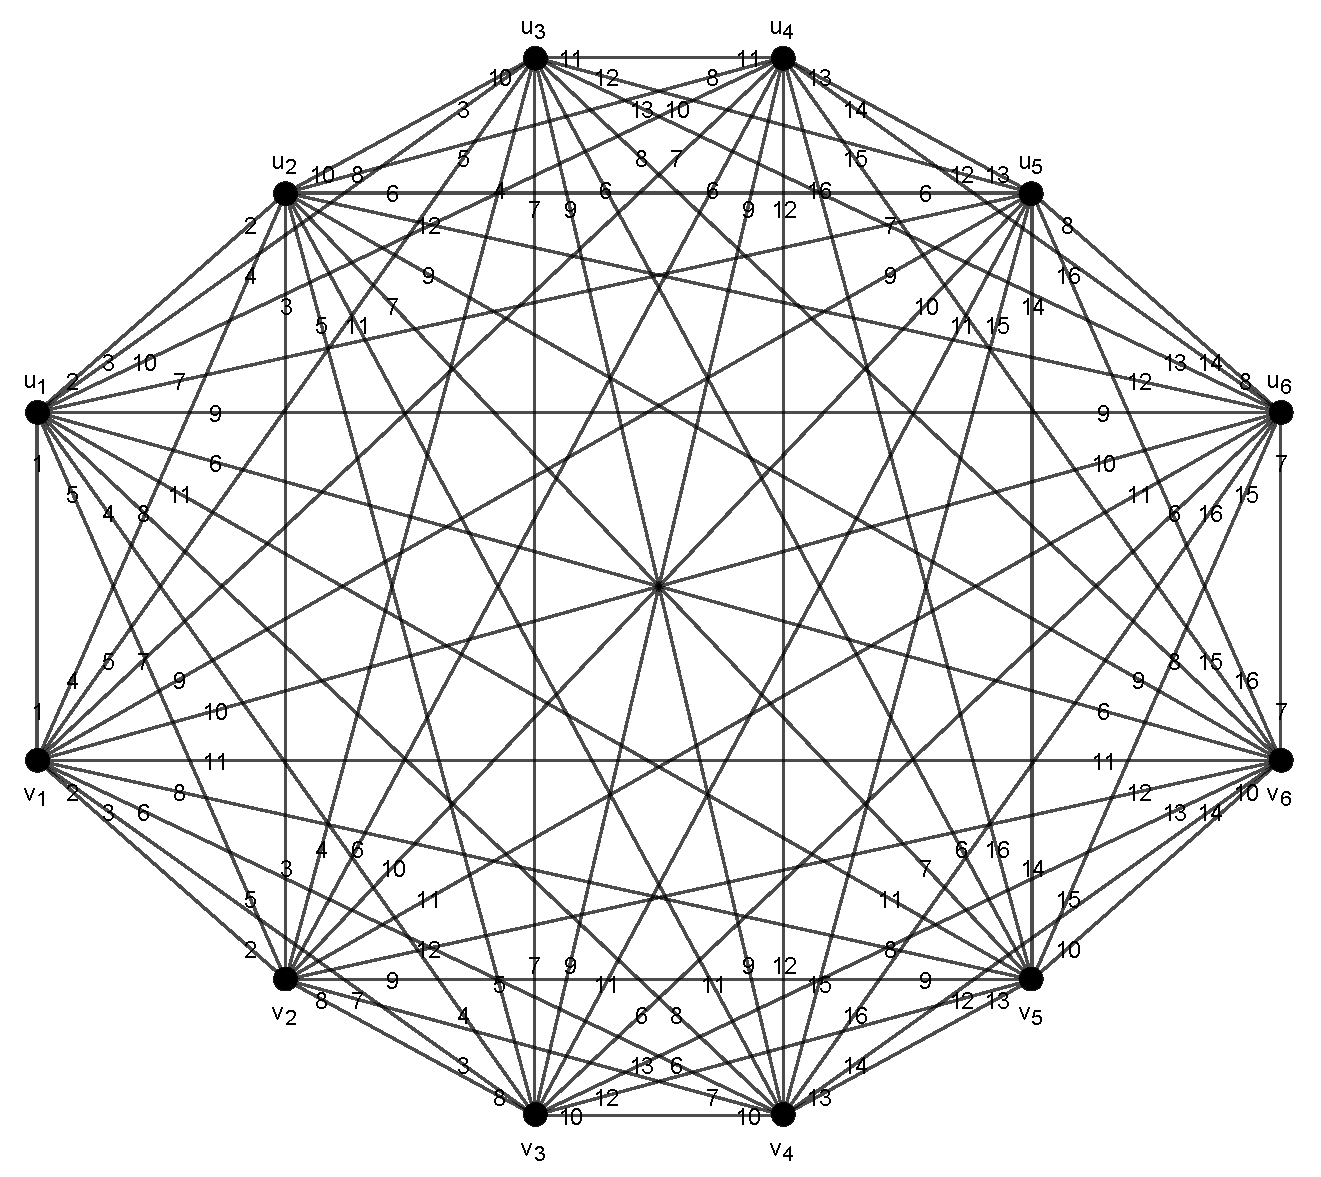
\includegraphics[width=0.7\textwidth]{figures/K_12-16.pdf}
\caption{$K_{12}$-ի միջակայքային $16$-ներկումը $(1,1,3,0,0)$ շեղման վեկտորով:}
\label{fK12}
\end{figure}


\begin{lemma}
\label{l2n6}
Եթե $\alpha$-ն $K_{2n}$-ի միջակայքային կողային ներկում է և $n\geq 9$, ապա  
$|{\rm sh}(\alpha)| \leq 2n-6$:
\end{lemma}
\begin{proof}[Ապացույց]
Ենթադրենք հակառակը՝ $|{\rm sh}(\alpha)| \geq 2n-5$: Լեմմաներ \ref{lReverse}-ից և \ref{l2k1}-ից հետևում է, որ $\sum\limits_{i=5}^{n-1}{b_i} \leq 2n-11$: Դիտարկենք երեք դեպքեր:
\begin{description}
\item{Դեպք 1.} $\sum\limits_{i=5}^{n-1}{b_i} = 2n-11$: Լեմմաներ \ref{lReverse}-ից, \ref{lBeforeSaturated}-ից և \ref{lAfterSaturated}-ից հետևում է, որ $b_{5} \geq 3$ և $b_{4} \leq 1$: Կիրառենք Լեմմա \ref{l2k1}-ը՝ տեղադրելով $k=3$, և ցույց տանք, որ $b_{1} + b_{2} + b_{3} = 5$ և $b_{4}=1$: Ապա կիրառենք Լեմմա \ref{lEdgeCount}-ը՝ տեղադրելով $k=3$: Անհավասարության ձախ մասը հավասար է $15$-ի: Աջ կողմում ունենք $\sum\limits_{i=1}^{3}{ib_i} \geq m(3,5)=12$ և $\sum\limits_{i=4}^{5}{(6-i)b_i} \geq 5$: Այս անհավասարությունները հակասում են Լեմմա \ref{lEdgeCount}-ին:

\item{Դեպք 2.} $\sum\limits_{i=5}^{n-1}{b_i} = 2n-12$: Լեմմա \ref{l2k1}-ից բխում է, որ $(b_1,b_2,b_3,b_4)$ վեկտորը հագեցած է: Լեմմա \ref{lAfterSaturated}-ից հետևում է, որ $b_5 \leq 1$: Հետևաբար, $(b_{n-1},b_{n-2},\ldots,b_6)$ վեկտորը հագեցած է և $b_5=1$: Լեմմա \ref{lBeforeSaturated}-ից բխում է, որ $b_6 \geq 3$: Այժմ կիրառենք Լեմմա \ref{lEdgeCount}-ը՝ տեղադրելով $k=4$: Անհավասարության ձախ մասը հավասար է $28$-ի: Աջ մասում ունենք, որ $\sum\limits_{i=1}^{4}{ib_i} \geq m(4,7)=20$ և $\sum\limits_{i=5}^{7}{(8-i)b_i} \geq 9$: Այս անհավասարությունները հակասում են Լեմմա \ref{lEdgeCount}-ին:

\item{Դեպք 3.} $\sum\limits_{i=5}^{n-1}{b_i} \leq 2n-13$: Լեմմա \ref{l2k1}-ից հետևում է, որ $\sum\limits_{i=1}^{4}{b_i} \leq 7$: Գումարելով այս երկու անհավասարուըյունները ստանում ենք հակասություն:
\end{description}
\end{proof}

\begin{figure}
\centering
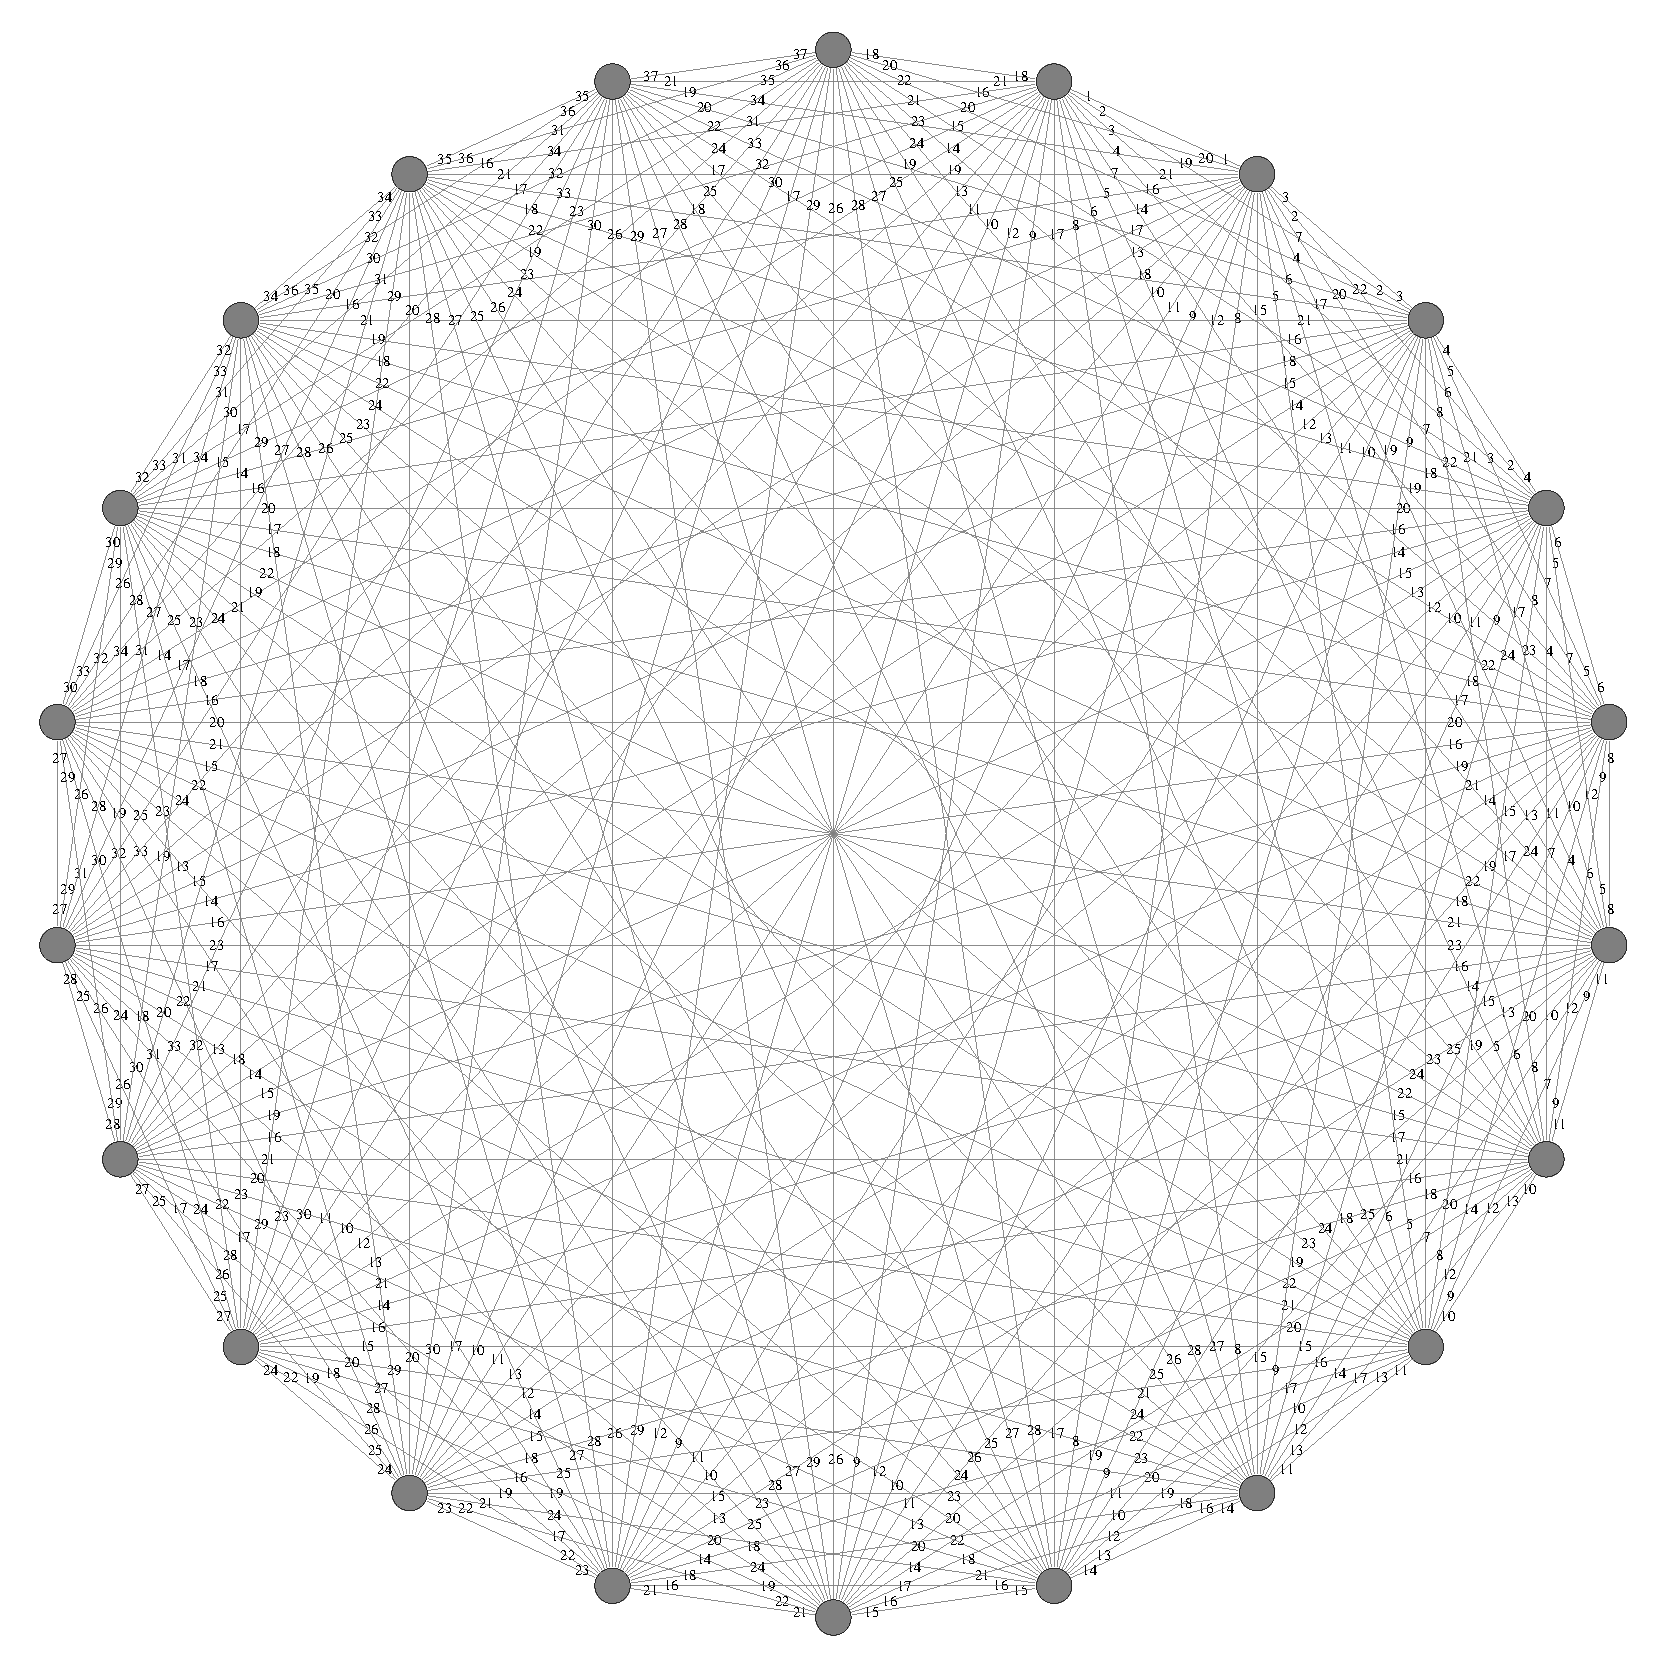
\includegraphics[width=\textwidth]{figures/K_22-37.pdf}
\caption{$K_{22}$-ի միջակայքային $37$-ներկում $(1,2,1,3,1,1,3,1,2,1)$ շեղման վեկտորով:}
\label{fK22}
\end{figure}


Հետևանքներ \ref{c2n4}-ից, \ref{c2n5}-ից, Լեմմա \ref{l2n6}-ից և Պնդում \ref{totalShift}-ից հետևում է $W(K_{2n})$-ի հետևյալ վերին գնահատականը:

\begin{theorem}
\label{tUpper}
Դիցուք $n \geq 3$:
\begin{center}
$W(K_{2n}) \leq \left\{
\begin{tabular}{ll}
$4n-5$, & երբ $n \geq 3$,\\
$4n-6$, & երբ $n \geq 5$,\\
$4n-7$, & երբ $n \geq 9$:\\
\end{tabular}
\right.$
\end{center}
\end{theorem}

Ստացված վերին գնահատականները թույլ են տալիս որոշել $W(K_{2n})$ պարամետրի ճշգրիտ արժեքները որոշ փոքր $n$-երի համար: Այդ արժեքները իրենց հերթին թույլ են տալիս լավացնել $W(K_{2n})$-ի ստորին գնահատականը, քանի որ Թեորեմ \ref{t1_lower}-ում ստացված գնահատականը կախված է $W(K_{2p})$ պարամետրի արժեքներից, որտեղ $p$-ն պարզ թիվ է: $p=2$ և $p=3$ դեպքերի համար $W(K_{2p})$-ի ճշգրիտ արժեքները հայտնի էին \cite{Petrosyan2010}-ից: $p=5$ դեպքում Թեորեմ \ref{t35n3}-ի ստորին գնահատականը համընկնում է Թեորեմ \ref{tUpper}-ի վերին գնահատականի հետ: $p=7$ դեպքը կլուծվի հաջորդ լեմմայում: Վերջապես, $p=11$ դեպքում Թեորեմ \ref{tUpper}-ի վերին գնահատականը հասանելի է $K_{22}$-ի միջակայքային $37$-ներկման միջոցով, որը պատկերված է Նկ. \ref{fK22}-ում: Այս ներկումը նաև հերքում է Հիպոթեզ \ref{h1_complete_log}-ը, ըստ որի $W(K_{22})=36$:

\begin{lemma}
\label{lK14}
$W(K_{14}) = 21$:
\end{lemma}
\begin{proof}[Ապացույց]
Թեորեմ \ref{tUpper}-ից հետևում է, որ $W(K_{14}) \leq 22$: Բավական է ցույց տալ, որ $K_{14}$-ը չունի միջակայքային կողային ներկում $22$ գույներով: Ենթադրենք հակառակը՝ գոյություն ունի $K_{14}$-ի $\alpha$ միջակայքային $22$-ներկում:

Դիտարկենք ներկման շեղման վեկտորը՝ ${\rm sh}(\alpha)=(b_1,b_2,b_3,b_4,b_5,b_6)$: Պնդում \ref{totalShift}-ից հետևում է, որ $\sum\limits_{i=1}^{6}{b_i}=9$: Լեմմա \ref{l2k1}-ից հետևում է, որ թե՛ առաջին և թե՛ վերջին եռյակի գումարը չի կարող գերազանցել $5$-ը: Առանց ընդհանրությունը խախտելու կարող ենք համարել, որ $b_1+b_2+b_3=5$ և $b_4+b_5+b_6=4$: Լեմմա \ref{lAfterSaturated}-ից բխում է, որ $b_4 \leq 1$: Լեմմաներ \ref{lReverse}-ից և \ref{l2k1}-ից հետևում է, որ $b_5+b_6=3$ և $b_4=1$: Ուստի $b_5 \geq 2$:

Այժմ ստուգենք Լեմմա \ref{lEdgeCount}-ի անհավասարությունը, երբ $k=3$: Ձախ մասը հավասար է $15$-ի: Աջ մասում ունենք, որ $\sum\limits_{i=1}^{3}{ib_i} \geq m(3,5) = 12$, $\sum\limits_{i=4}^{5}{(6-i)b_i} \geq 4$: Գումարելով այս անհավասարությունները ստանում ենք հակասություն:
\end{proof}

Լավագույն ստորին գնահատականը, որը հաջողվել է ստանալ, հետևյալն է: 

\begin{theorem}
\label{t1-complete-W-lower-best}
Եթե $n = \prod\limits_{i=1}^{\pi(n)}{p_i^{\alpha_i}}$, որտեղ $p_i$-ն $i$-րդ պարզ թիվն է, $\pi(n)$-ը՝ $n$-ը չգերազանցող պարզ թվերի քանակը, իսկ $\alpha_i \in \mathbb{Z}_{\geq 0}$, ապա
\begin{center}
$W(K_{2n}) \geq 4n - 3 - A_n$,
\end{center}
որտեղ $A_n = \alpha_1 + 2\alpha_2 + 3\alpha_3 + 4\alpha_4 + 4\alpha_5 + \frac{1}{2}\sum\limits_{i=6}^{\pi(n)}{\alpha_i(p_i+1)}$:
\end{theorem}
\begin{proof}[Ապացույց]
Թեորեմն ապացուցելու համար վերցնենք Թեորեմ \ref{t1_lower}-ի ստորին գնահատականը, տեղադրենք $W(K_{2p_i})$-ի ճշգրիտ արժեքները առաջին հինգ պարզ թվերի համար, իսկ $W(K_{2p_i})$ թվերը, $i\geq 6$, գնահատելու համար կիրառենք Թեորեմ \ref{t35n3}-ը՝ հաշվի առնելով, որ բացի $2$-ից բոլոր պարզ թվերը կենտ են:
\end{proof}

Այս Թեորեմից և Թեորեմ \ref{t1_regular}-ից ստանում ենք հետևյալ արդյունքը.
\begin{corollary}
Եթե $n = \prod\limits_{i=1}^{\pi(n)}{p_i^{\alpha_i}}$, որտեղ $p_i$-ն $i$-րդ պարզ թիվն է, $\alpha_i \in \mathbb{Z}_{\geq 0}$, $\pi(n)$-ը՝ $n$-ը չգերազանցող պարզ թվերի քանակը, իսկ $2n-1 \leq t \leq 4n - 3 - A_n$, որտեղ $A_n = \alpha_1 + 2\alpha_2 + 3\alpha_3 + 4\alpha_4 + 4\alpha_5 + \frac{1}{2}\sum\limits_{i=6}^{\pi(n)}{\alpha_i(p_i+1)}$, ապա $K_{2n}$-ը ունի միջակայքային $t$-ներկում:
\end{corollary}


Այսպիսով, հայտնի են $W(K_{2n})$-ի ճշգրիտ արժեքները, երբ $n \leq 12$ և $n=16$: Այդ արժեքները, ինչպես նաև հայտնի լավագույն ստորին և վերին գնահատականները ներկայացված են Աղյուսակ \ref{tableAll}-ում:

\begin{table}[h]
\centering
\begin{tabularx}{0.96\textwidth}{r||*{18}{c<{\hspace{-1.2pt}}|}}
$n$ 
& $1$ & $2$ & $3$ & $4$ & $5$ & $6$ & $7$ & $8$ & $9$ & $10$ & $11$ & $12$ & $13$ & $14$ & $15$ & $16$ & $17$ & $18$ \\ \hline\hline
$W(K_{2n}) \geq $ 
& $1$ & $4$ & $7$ & $11$ & $14$ & $18$ & $21$ & $26$ & $29$ & $33$ & $37$ & $41$ & $42$ & $46$ & $52$ & $57$ & $56$ & $64$ \\ \hline
$W(K_{2n}) = $
& $1$ & $4$ & $7$ & $11$ & $14$ & $18$ & $21$ & $26$ & $29$ & $33$ & $37$ & $41$ &  &  &  & $57$ &  &    \\ \hline
$W(K_{2n}) \leq $
& $1$ & $4$ & $7$ & $11$ & $14$ & $18$ & $22$ & $26$ & $29$ & $33$ & $37$ & $41$ & $45$ & $49$ & $53$ & $57$ & $61$ & $65$
\end{tabularx}
\caption{
	$W(K_{2n})$-ի գնահականները: Առաջին տողում բերված են ստորին գնահատականները ըստ Թեորեմ \ref{t1-complete-W-lower-best}-ի, երկրորդ տողում հայտնի ճշգրիտ արժեքներն են, իսկ երրորդ տողում վերին գնահատականներն են ըստ Թեորեմ \ref{tUpper}-ի:
}
\label{tableAll}
\end{table}

2016թ. Հուդակը, Կարդոշը, Մադարասը և Վրբյարովան \cite{HudakEtAl2016} դիտարկել են լրիվ գրաֆների միջակայքային ներկումների մի տարատեսակ, որտեղ ներկման ճշտությունը չի պահանջվում: Մասնավորապես, հեղինակները ցույց են տվել, որ այդ դեպքում ներկմանը մասնակցող առավելագույն գույների քանակը գագաթների թվից կախված խիստ աճում է: 